%%%%%%%%%%%%%%%%%%%%%%%%%%%%%%%%%%%%%%%%%%%%%%%
%
% Template per Elaborato di Laurea
% DISI - Dipartimento di Ingegneria e Scienza dell’Informazione
%
% update 2015-09-10
%
% Per la generazione corretta del
% pdflatex nome_file.tex
% bibtex nome_file.aux
% pdflatex nome_file.tex
% pdflatex nome_file.tex
%
%%%%%%%%%%%%%%%%%%%%%%%%%%%%%%%%%%%%%%%%%%%%%%%


% formato FRONTE RETRO
\documentclass[epsfig,a4paper,11pt,titlepage,twoside,openany]{book}
\usepackage{import}
\usepackage{preamble}

\begin{document}
  % nessuna numerazione
  \pagenumbering{gobble}
  \pagestyle{plain}

\thispagestyle{empty}

\begin{center}
  \begin{figure}[h!]
    \centerline{\psfig{file=images/marchio_unitrento_colore_it_202002.eps,width=0.6\textwidth}}
  \end{figure}

  \vspace{2 cm}

  \LARGE{Dept. of Information Engineering and Computer Science\\}

  \vspace{1 cm}
  \Large{Master's Degree in\\
	Computer Science
  }

  \vspace{2 cm}
  \Large\textsc{Final Dissertation\\}
  \vspace{1 cm}
  \Huge\textsc{Quieting the noise in the Internet Inter Domain Protocol\\}
  \Large{\it{A simulation based study of BGPs noise reduction mechanisms and their interaction}}


  \vspace{2 cm}
  \begin{tabular*}{\textwidth}{ c @{\extracolsep{\fill}} c }
  \Large{Supervisors} & \Large{graduating student}\\
  \Large{Prof. Renato Lo Cigno}& \Large{Milani Mattia}\\
  \Large{Prof. Timothy G. Griffin (Univ. of Cambridge)}\\
  \end{tabular*}

  \vspace{2 cm}

  \Large{Accademic Year 2019/2020}

\end{center}



  \clearpage

  \thispagestyle{empty}

\begin{center}
  {\bf \Huge Thanks}
\end{center}

\vspace{4cm}


\emph{
  ...thanks to...
}

  \clearpage
  \pagestyle{plain} % nessuna intestazione e pie pagina con numero al centro

  % inizio numerazione pagine in numeri arabi
  \mainmatter

  % indice
  \tableofcontents
  \clearpage

  % gruppo per definizone di successione capitoli senza interruzione di pagina
  \begingroup
    % redefinizione del formato del titolo del capitolo
    % da formato
    %   Capitolo X
    %   Titolo capitolo
    % a formato
    %   X   Titolo capitolo

    \titleformat{\chapter}
      {\normalfont\Huge\bfseries}{\thechapter}{1em}{}

    \titlespacing*{\chapter}{0pt}{0.59in}{0.02in}
    \titlespacing*{\section}{0pt}{0.20in}{0.02in}
    \titlespacing*{\subsection}{0pt}{0.10in}{0.02in}

    % sommario
    \chapter*{Summary} % senza numerazione
\label{cha:summary}

\addcontentsline{toc}{chapter}{Summary} % da aggiungere comunque all'indice

...summary....





    \chapter{Introduction}
\label{cha:introduction}

%\begin{itemize}
%    \item How is internet built
%    \item the protocol that controls internet
%\end{itemize}

%\fxfatal{Expand the concepts}

What we call the Internet is a single network that interconnects more than \num{60000}
\acp{AS} that share their knowledge to spread the sub-nets reachability.
An \ac{AS} is a single entity that holds and controls some \textit{IP} prefixes
used by one or more operators.
Every \ac{AS} is responsible for its own inter-connectivity policies that control
the spread of information obtained by the outside and the one from the inside.

The \ac{BGP} is the only protocol used on the Internet that controls the propagation
of the knowledge between different \acp{AS}.
\ac{BGP} has been released in \num{1989} and is in use on the internet since
\num{1994}.
Since that year \ac{BGP} is growth a lot, it reached its last version, number
fourth, in \num{2006} \cite{rfc4271}.
Up to now, \ac{BGP} can be expanded with tens of \acp{RFC} that extends the
range of possibilities,
from policies to attributes used to tag messages and give more information than
just the path to reach the destination.

Multiple of its parameters play a central role in it, and the correct setting
of them could influence the performances of, not only the single \ac{AS} but
the entire network.
For this reason, the research is still active to find new technologies and
a trade-off between, convergence time and messages transmitted.

In this thesis, more precisely in \Cref{cha:bgp_art}, I'm going to introduce
two of them, \ac{MRAI}, used to compress multiple input messages into one
output message and the \ac{RFD} parameter, that is used to penalize unstable paths
suppressing routes.
Those two parameters goal is to control two different types of noise that
\ac{BGP} creates/suffers.

The existence of those two parameters has been studied separately many different
times \cite{fabrikant2011there,daggitt2018rate,qiu2005optimal,gray2020bgp}.
But, there are almost no studies on the correlation of those parameters.
Even if the effects of one interact with the other.

\section{Internet today}
\label{sec:internet_today}

Internet, as a network, is constantly growing, in terms of \acp{AS}, prefixes
and messages transmitted.
Increasing also the load on the \ac{BGP} nodes and by consequence the load
of the network in general.
There are constantly smaller prefixes announced, the number of $/24$ prefixes
distributed in the last years has been growing constantly.
Data obtained from the annual report of the \ac{AS} 131072 that register the
evolution of its node since \num{2007} from two \ac{BGP}
speakers point of the \ac{APNIC}, one located in Japan and the other in
Australia\footnote{\href{https://blog.apnic.net/2021/01/05/bgp-in-2020-the-bgp-table/}{source APNIC data}}.

This growth of the Internet is not negligible because of one, between the may,
problem that it has due to the \ac{BGP} protocol.
\ac{BGP} suffers from the \textit{Path Exploration} problem, a node can enter in
a transitory state where it continuously shares non-optimal paths while it
doesn't reach a stable state.
Even few tens of nodes can generate thousands of messages due to this problem
\cite{deshpande2004impact}.
And this problem cannot be overloked on a \num{60000} nodes network that we all
rely on every day.

\section{Correlation between variables and convergence}
\label{sec:bgp_correlations}

The two parameters that will be studied in this thesis are \ac{MRAI} and \ac{RFD}
and how the interaction between them works.
Our first hypothesis is that, indeed, there is an interaction.
This hypothesis is sustained by the fact that both parameters operate to
control the noise of \ac{BGP}, with different parameters and different behaviour,
but, if a node wants to transmit a message it must respect \ac{MRAI} and the input
could be caused by \ac{RFD} that suppress/reintroduce a route.
On the opposite case, a too small \ac{MRAI} value could permit different message
storms that would trigger the \ac{RFD} suppression systems creating vicious circle.

One of the goals of reducing the value of \ac{MRAI} is to reach a faster convergence
paying the cost of more messages.
Unfortunately, looking only to \ac{MRAI} is not possible to get reliable results
for general purposes, in-fact, like showed in \Cref{cha:bgp_rfd}, is possible
to obtain the opposite result due to the fact that to solve \ac{RFD} suppression
is required a longer time.

On the opposite case if we tune in the wrong way \ac{RFD} we would end up to
be too much permissive, leaving to handle all the noise to \ac{MRAI} that could
be not effective if the storms are sufficiently delayed in time.

For those reasons is important to study these two parameters together, because
there could be a strong co-dependence.

\section{The goal of this thesis}
\label{sec:thesis_goal}

%\begin{itemize}
%    \item Why is important understand this correlation?
%\end{itemize}

The goal of this thesis is to prove that the noise detectors of the \ac{BGP}
protocol are correlated, studying this correlation through stimulative experiments
and from those give useful hints on how those two parameters interact with one another.
In order to build the basis for future experiments that can study more deeply
and maybe in a formal way the phenomena.
Is also mandatory for this thesis to develop the platform where those experiments
would be executed and make that platform public
available\footnote{\href{https://github.com/tiamilani/BGPFSM}{GitHub repository}}.

In \Cref{cha:bgp_art} are going to be presented the protocol and more deeply
the two parameters studied, while in \Cref{cha:des} I'm going to present
the structure of the platform that will be used in \Cref{cha:bgp_fsm,cha:bgp_mrai_experiments,cha:bgp_rfd}
to perform the experiments about the \textit{Path Exploration} problem and then
how \ac{MRAI} and \ac{RFD} can impact the performances, conclusions to follow
in \Cref{cha:conclusion}.

The \ac{BGP} community has not yet reached a common agreement on what values
to use for this reason I will evaluate different possible techniques that can
be applied to both the parameters and comment on the network performances obtained.


    \chapter{BGP state of the art}
\label{cha:bgp_art}

\ac{BGP} is the protocol used to control the information spreading on the Internet.
It is currently at version \num{4}, published in \num{2006} with the \ac{RFC} \num{4271}
\cite{rfc4271}.
\ac{BGP} is a \ac{PV} protocol, it distinguishes itself from the \ac{DV} and \ac{LS}
protocols with the major difference that it shares other than the knowledge of
a path also the path itself to reach the destination.

\ac{BGP} has two major sub-categories with a difference in the flow of information
direction:
\begin{itemize}
	\item \textbf{\textit{\ac{eBGP}}:} I will talk about \ac{eBGP} when the
		flow of information goes from the inside
		of the \ac{AS} to other \acp{AS};
	\item \textbf{\textit{\ac{iBGP}}:} I will talk about \ac{iBGP} when the flow
		of information goes from the outside of the \ac{AS} to the inside of
		it, to make aware of the new routes also the internal routing protocol.
\end{itemize}

My main interest in this thesis is for the \ac{eBGP} part of the protocol, for
now on I will refer to it talking in general of \ac{BGP} without further distinguishing
from the internal protocol.

When there is an interconnection between two \acp{AS} that creates a \ac{BGP}
link, I will talk about peering referring to the connection, and those \ac{BGP}
speakers interconnected will be the peers.
Each \ac{BGP} link is based on a direct \ac{TCP} connection.
On these links, every \ac{AS} can configure its own policies that would be used
to evaluate routes at the reception or in the moment there is something new
to share.
There are three different possible type of relations that can be created by two
\ac{BGP} speaker, accordingly to the \ac{CAIDA}:

\begin{itemize}
	\item \textbf{\textit{\ac{c2p}}:} This relationship highlights the fact that
		lower \ac{AS} pays a higher level \ac{AS} to get connectivity and access
		to the Internet;
	\item \textbf{\textit{\ac{p2p}}:} This relationship is used to share the knowledge
		between two \acp{AS} of their customer providers without paying a higher
		level \ac{AS};
	\item \textbf{\textit{\ac{s2s}}:} This relationship defines the connection
		between \acp{AS} under the same \ac{ISP}.
\end{itemize}

During this thesis, I will only consider the first two relationships \ac{c2p} and
\ac{p2p}, the schema in \Cref{fig:AS_flow} shows how the traffic is affected
based on the type of the link crossed.

\begin{figure}[ht]
    \centering
    \includegraphics[scale=0.75]{images/BGP/ASKnowledgeDistribution.pdf}
	\caption{Distribution schema for the \acp{AS}, the row colours distinguish
	different flows, $AS\_X$ is a customer of the servicer set, a peer with the
	peers set and servicer for the customers set}
    \label{fig:AS_flow}
\end{figure}


As shown by the flows with a different colour in \Cref{fig:AS_flow} a single
\ac{AS} will share information considering the receiving link.
If something comes from one of its customers it will share the knowledge with
every other link that it has, even other customers (always respecting the output policies).
If a route has come from its provider or a peer then it will be only shared with
its own customers.
Those policies are commonly called \q{valley-free} and are dictated by convenience,
an \ac{AS} has all the advantages when
other \acp{AS} decide to use it to reach a specific destination.
For this reason is convenient for an \ac{AS} that everyone knows about its clients
networks, and, in the opposite side, that its clients knows only the route
through it to reach other networks.

This behaviour can be modelled with a variant of the \ac{SSP} algebra described
in \cite{daggitt2018rate}.
This is the same algebra that will be used in \Cref{cha:des} to describe the links
relationships.

%\begin{itemize}
%    \item BGP de facto standard on the internet
%    \item What is an AS
%    \item interconnection between ASes
%\end{itemize}

\section{The protocol in details}
\label{sec:bgp_intro}

Once a \ac{BGP} node has established a connection with another peer it will
start to exchange routes with that neighbour, always respecting the policies.
Its important to underline that, a \ac{BGP} speaker only shares its best routes
and in this protocol the best decision is dictated by the policies, and
then other possibilities would be evaluated (number of hops, bandwidth etc).
For this reason the best path decided by a node could differ from the actual
best path from a topological point of view.

Every \ac{BGP} node has a \ac{RIB} as data structure to keep the information
about the received routes, the alternative routes and what should be exported.
The \ac{RIB} is divided into \num{3} sections.
\begin{itemize}
	\item \textbf{\textit{ADJ-RIB\_in}:} This \ac{RIB} contains all the routes
		that have been received by other \ac{AS} in order to be evaluated;
	\item \textbf{\textit{LOC-RIB}:} This \ac{RIB} contains all the best routes
		that have been chosen from the \textit{ADJ-RIB\_in} from the node;
	\item \textbf{\textit{ADJ-RIB\_out}:} There is an output \ac{RIB} for every
		neighbour of the node, it contains the route that should be advertised
		to the specific node.
\end{itemize}

One of the most important parts of \ac{BGP} is its decision process, that would
be applied to discern between the routes in the \textit{ADJ-RIB\_in} in order
to update the \textit{LOC-RIB} and, if necessary also the \textit{ADJ-RIB\_out}.
The decision process is composed of three parts:
\begin{itemize}
	\item[1] Calculation of the preference: This function is called every time
		there are new reachability information that needs to be evaluated, it
		will assign/update the preference value at every route in the
		\textit{ADJ-RIB\_in} using policy filters pre-configured. If a route
		doesn't respect the policy filters it will be then marked as ineligible,
		otherwise, a \textit{PREF\_VALUE} will be calculated and assigned to the
		route;
	\item[2] Route selection: This function is called at the end of the first
		phase, it collects all the eligible routes and evaluates them removing
		routes that would create loops or that creates conflicting situations.
		The evaluated routes are then ordered by the \textit{PREF\_VALUE} and
		then the best route will be then installed in the \textit{LOC-RIB}.
		In case of ties, there is an algorithm that can be used to break them;
	\item[3] Route dissemination: This function can be called in different
		situations, it will use the information in the \textit{LOC-RIB} to
		populate every \textit{ADJ-RIB\_out}, according to configuration
		policy.
\end{itemize}
The decision process is also responsible for the route aggregation and information
reduction.
At the end of the third phase, the \ac{BGP} speaker will execute the
\textit{Update-send} process, that is responsible for the effective dissemination.

There are multiple types of packets that can be sent by a \ac{BGP} speaker, but
I will focus only on the \ac{ADV} packets.
The \ac{ADV} packets are responsible for the dissemination of the information
to other nodes that will analyze and use the attribute inside the message
to assign a preference value to the route.
In particular, there are two sections of the \ac{ADV} messages that will
contain additive information and subtractive information.
Is possible to distinguish \ac{ADV} messages using the type of information that are
transmitting:
\begin{itemize}
	\item \textbf{\textit{UPDATE}:} This type of messages represent the distribution
		of new reachability information, a new best route to a destination will be
		shared through an update message;
	\item \textbf{\textit{WITHDRAW}:} This type of messages are distributed when
		a node want to share that it doesn't know how to reach
		a destination anymore.
\end{itemize}
Inside those packets, there are different attributes that permit to transfer
information about the route (advertised or withdrawn).
There is an attribute that describes the address that the route represents,
another one that contains the path that will be used to reach the
destination, the next-hop used, etc.
During the years multiple new \ac{RFC} have introduced, modified, updated and removed
attributes that can be found inside an advertisement message.
Not all the attributes are mandatory for \ac{BGP} nodes, in fact, for a node
is possible to receive a route with an attribute that it is not able to interpret
but (if configured to do so) it will share the route with also the unknown
attributes.

Is important to remember that all those information are useful for the policy
filters that every node can have, for example, some nodes would automatically discard
any route that contains a specific \ac{AS} in the received path.

The \textit{Update-send} process is responsible for the distribution of the
messages that are stored in the \textit{ADJ-RIB\_out}.
It execute again some checks on the \ac{RIB}, removing unfeasible routes
and removing routes that have already been advertised to the pear.
It also has to respect a temporal constraint, introduced in \cite{rfc4271},
a \ac{BGP} speaker can't send to the same neighbour routes for the same destination
more often than the \ac{MRAI} value.
\ac{MRAI} act as a timer whose goal is to avoid continuous update storm caused
by decision changes in some peers in the network.

Another property that can be found in \ac{BGP} nodes, that affects the messages
transmitted, is the \ac{IW}.
This property permits to reduce the number of messages that are distributed.
Without this option when a \ac{BGP} node discovers a new best path to reach
a destination should send a withdraw followed by an update to its neighbourhood.
Thanks to this option is sufficient to send just the update, the other nodes
will learn that the best path is changed simply looking to the previous
alternative and comparing them.

%\begin{itemize}
%    \item High level of BGP
%    \item BGP messages
%    \item BGP Update messages
%    \item BGP policies
%	\item two type of BGP noise, the one caused by BGP itself and the one
%		caused by flapping interfaces
%\end{itemize}

%\section{BGP Wedgies}
%\label{sec:bgp_wedgies}
%
%\begin{itemize}
%    \item What are wedgies?
%    \item why are them important?
%    \item which situations them occur?
%\end{itemize}

\section{BGP inherent noise vs external noise}
\label{sec:bgp_noise}

With the term \textit{BGP Noise} I define a particular behaviour
of \ac{BGP}.
It underlines a situation where the nodes are distributing routes
that would be retrieved few moments later.
Non optimal messages are shared while nodes don't have a compleate knowledge
to take the best possible solution, producing multiple \ac{ADV} storms.
This behaviour is defined as noise because of the tendency of \ac{BGP} to act
as an echo-chamber amplifying this distribution of incorrect information.
%All those wrong messages are going to disturb the convergence of the protocol.
In fact, a \ac{BGP} node that receives an update from a neighbour will probably
redistribute the route to multiple neighbours, peers and servicer.
Given the hierarchical topology of the internet this behaviour grows
exponentially while the information reach the center of the network.

There are basically two sources of noises in \ac{BGP}, the inherent noise of
the protocol and the noise caused by external sources.
Those two type of noises are triggered by different causes and are
not discernible one another.
Because, both the noise situation are characterized by an intense distribution
of messages and there are no other distinguishing features.

The first one is caused by the protocol itself when it tries to converge
on new knowledge.
The sharing of new routes can cause new \ac{ADV} that can then trigger the
\textit{Path Exploration} problem.
This is a noise caused by the protocol itself that distribute \ac{ADV} for
new paths that will change until the best possible path is taken in consideration.

One \ac{BGP} parameter tries to limit this noise acting as a message cache with
a compression system.
This parameter is \ac{MRAI} and it permits to avoid sending a message for every
new one received using a timer.
Only the best decision after that delay will be shared.

The second type of noise is caused by a source outside the protocol.
A miss-configuration or a faulty interface can cause the transmission of not necessary messages.
For example, the withdraw and the advertisement of a route at a continuous interval.
This type of behaviour will cause continuous storms of messages and the triggering
of the first noise type.
Also, the transmission of a withdraw followed by an announcement is considered
a \q{flap}.

\ac{BGP} introduce a parameter with the \ac{RFC} \num{2439} \cite{rfc2439} that
is called \ac{RFD} to overcome this behaviour.
This parameter increases a value every time a flap or a route change is detected,
when this value passes a predefined threshold the route will be suppressed.
This value will always decay using an exponential decay function, even if it
doesn't overpass the threshold.
The decay function is calculated defining the time that the function should take
to half the value, by default \SI{15}{\minute}.
Once the route has been suppressed the \ac{BGP} speaker must wait enough time
that the value goes below another indicator before sharing it again.

Those two parameters are clearly connected one another from the fact that
one triggers the other and vice versa, is possible to create a particular topology
that has different performances based on the values assigned to those
parameters.
Think about two clique networks connected one another by only one node, that
node will act as a bottleneck, probably its \ac{RFD} threshold would be easily
overpassed and then it depends on its decay function before it can share
again the prefix to the second clique triggering \ac{MRAI} on those nodes that
will experience the path exploration problem.

%\fxfatal{I think that the graphs in Fig 2 and Fig 3 of Fabrikant et al. in
%\cite{fabrikant2011there} will easily trigger both \ac{MRAI} and \ac{RFD}}

\section{BGP MRAI, designed to reduce inherent noise}
\label{sec:bgp_mrai}

\ac{MRAI} is one of the parameters that mostly affect the convergence of \ac{BGP}.
A high value of it could unnecessarily delay the transmission of messages, but,
in the opposite case, a value too small can provoke a lot of messages, one for
every decision change of the node.
The main function of it is to reduce the intrinsic noise of \ac{BGP} compressing
the set of messages received.
There are a lot of studies about it, and it has already been shown that
the number of messages and the convergence time can depend on it~\cite{griffin2001experimental}.
Also, it has been already proven by Fabrikant, Rexford et al.~\cite{fabrikant2011there}
that an incorrect configuration of it could lead to tremendous consequences.

\ac{MRAI} has been introduced in the \num{4}Th version of \ac{BGP}~\cite{rfc4271} and
it is nowadays a mandatory mechanism for every \ac{BGP} node, otherwise the load
in terms of messages to process and decision changes would be incalculable.
Its main purpose, as anticipated in \Cref{sec:bgp_noise}, is to prevent or
at least mitigate the noise created by \ac{BGP} itself.

The most important component of \ac{MRAI} is a timer that controls how much time must pass
between one \ac{ADV} and the following one.
The timer is peer-based, for each interconnection an \ac{AS} could have a different
\ac{MRAI}, but it acts for every destination in parallel, this means that there
is a different timer for each destination that a node would share for every
\ac{BGP} relations that it has.
The idea behind it is that, in the period of time between one \ac{ADV} and the
following one the \ac{BGP} node will be able to receive other possible routes.
The enriched set of possibilities would give to the speaker the ability to take
a decision closer to the absolute best.
\ac{MRAI} has the property to compress the input messages sequence in order to have
an output message sequence with a smaller number of \ac{ADV}.

The behaviour of a \ac{BGP} node with \ac{MRAI} is defined as follow for every
change in the \textit{ADJ-RIB\_out} of a neighbour caused by the
\textit{Update-send} process:
\begin{itemize}
	\item If there isn't an active \ac{MRAI} timer for the destination changed
		send the \ac{ADV} and set an \ac{MRAI} timer;
	\item If there is an active \ac{MRAI} timer for the destination then
		don't send anything;
	\item When the active \ac{MRAI} timer ends if there is still the necessity
		to send an \ac{ADV} then send it and set another \ac{MRAI} timer.
\end{itemize}

The second passage permits the route selection process to be executed multiple
times before the actual transmission of the decision.
That because \ac{MRAI} limits only the transmission and not the decision process.
The condition to the last passage is due to the fact that the compression some
times could lead to the not necessity to actually send a message.

The default value defined in the \ac{RFC} \num{4271} for \ac{MRAI} is equal to
\SI{30}{\second}.
But, \ac{MRAI} is a really controversial parameter, it has received multiple
revisions and studies.

In \num{2008}, thanks to different studies that take into consideration the
dimension of the topology and the latency~\cite{qiu2005optimal}, there has been
the proposal to reset its default value to \SI{5}{\second}~\cite{jakma2008revised}
In \num{2010}, a proposal \ac{RFC} of the \ac{IETF}~\cite{jakma2010revisions}
says that the default value would be left to the arbitrary choice of the operators and
that withdraw message could completely ignore it.
But, this freedom would damage the convergence and the number of messages distributed
as showed by Fabrikant et al.~\cite{fabrikant2011there}.

Is clear that \ac{MRAI} affect the network performances, but what affects \ac{MRAI}
and, by consequences, the performances?
Obviously, the choice itself of a different \ac{MRAI} strategy can have a huge
impact, as showed for example in~\cite{milani2019BGP}, where the centrality
has been used to obtain better results in the case of network faults.
But, giving the fact that, the main function of \ac{MRAI} is to compress the
input messages, also the sequence of messages receipt could be meaningful.
Giving that \ac{MRAI} is a link-based parameter also the number of links that
a node has could influence it and by consequences the position in the topology.
A well connected node will be more likely to receive multiple paths and messages
than one with only one link.

\section{BGP RFD, designed to reduce external noise}
\label{sec:bgp_rfd}

\ac{RFD} is a parameter introduced in \ac{BGP} to overcome the problems caused
by exterior sources of noise.
It main function is to avoid the computation overload provoked by fluctuating
routes with continuous message storms.
It has been introduced with the \ac{RFC} \num{2439} in \num{1998}~\cite{rfc2439}.
Also, \ac{RFD} is a controversial parameter, it has been studied and evaluated again
different times, but, recent studies showed that the majority of the operators
still use deprecated values from \num{2001}~\cite{gray2020bgp}.
Furthermore, other studies show that the majority of the \ac{ADV} that travels
through the Internet are generated by a restricted set of \acp{AS}, but \ac{RFD}
seems to be too much restrictive and affect the majority of the \acp{AS} traffic~\cite{pelsser2011route}.

\ac{RFD} will use a single value, called \textit{figure of merit}, to evaluate
the actual situation of a route, while this value evolves the \ac{RFD} algorithm
will make a decision on what to do.
The evolution of the \textit{figure of merit} is dictated by the messages received,
with fluctuations it will grow, while, over time, it will use a quadratic decay
function to decrease.
Fluctuations, or flaps, are represented by the reception of the withdraw and
the announcement of a route, a path change is also considered a flap, even
if thanks to \ac{IW} is limited to just one \ac{ADV}.

There are other parameters that are part of this \ac{BGP} component, the more
important are presented in \Cref{tbl:rfd_defaults}.

\begin{table}[ht]
	\begin{center}
	\begin{tabular}{ || m{5cm} | m{4cm} | m{4cm} || }
	\hline
			Parameter & Cisco default values & Juniper default values\\
	\hline \hline
			withdrawal penalty & 1.0 & 1.0 \\
	\hline
			re-advertisement penalty & 0.0 & 1.0 \\
	\hline
			attribute change penalty & 0.5 & 0.5 \\
	\hline
			suppress threshold & 2.0 & 3.0\\
	\hline
			half-life (min) & 15 (900s) & 15 (900s)\\
	\hline
			Reuse Threshold & 0.75 & 0.75 \\
	\hline
			Max Suppress Time (min.) & 60 (3600s) & 60 (3600s)\\
	\hline
	\end{tabular}
\end{center}

		\caption{\ac{RFD} parameters}
	\label{tbl:rfd_defaults}
\end{table}

Other than the name of the parameters, in \Cref{tbl:rfd_defaults} is showed also
the default value decided by Cisco and Juniper.
The \ac{RFC} \num{2439}~\cite{rfc2439} gives some guidelines on how to set those
values but the actual choice is left to the discretion of implementors.
The first three parameters, \textit{Withdraw, re-advertisement, attribute change}
represent the penalty applied to the \textit{figure of merit} when the homonym event
happen.
The \textit{suppression threshold} represents the level at which the \ac{BGP} node will
suppress the route and don't advertise it until the figure of merit goes
below the \textit{reuse threshold}.
The decay of the \textit{figure of merit} follows a quadratic decay function
which rate is calculated using the \textit{Half-life} parameter.
The \textit{Max Suppress Time} will override all this parameters because, as
defined in the original \ac{RFC}, a route cannot be suppressed for more than
that time, it doesn't matter the figure of merit accumulated by this route.

An example of the figure of merit evolution could be seen in \Cref{fig:figure_of_merit},
This image has been taken from \cite{gray2020bgp}.

\begin{figure}[ht]
    \centering
    \includegraphics[scale=0.22]{images/RFD/evolution.png}
	\caption{Example of evolution of the \ac{RFD} \textit{figure of merit} taken
	from \cite{gray2020bgp}, yellow messages represent withdraws and green ones
	are advertisement, the dashed lines are the suppression and reuse threshold}
    \label{fig:figure_of_merit}
\end{figure}

\Cref{fig:figure_of_merit} shows a hypothetic evolution of the \ac{RFD} filter,
it doesn't rely on the default value of the Cisco or Juniper implementation.
Is possible to see, in the lower part of the plot, the messages received by the
\ac{BGP} speaker, yellow one represent withdraws while the green are announcements.
Is possible to see that the penalty value grows at each flap and as soon it reaches
the suppression threshold the route will not be advertised to any neighbour.
While after the decay has reached the reuse level is possible to advertise the
route again.

Is possible to see that \ac{RFD} doesn't make any difference on its own on what
is causing the flaps, it simply constant reacts to the evolution of the network.
Is not even possible to determine where is located the flap, if the source
is flapping heavily for some reasons or there is an \ac{AS} in the middle of the
path that is malfunctioning.

\ac{RFD} has a troubled history, maybe even more than \ac{MRAI}.
In \num{2006}, thanks to the publication of \cite{mao2002route}, the \ac{RIPE}
recommends to disable it\cite{smith2006ripe}.
A few years later, after the publication of the article from Pelsser et al.~\cite{pelsser2011route}
\ac{RIPE} and \ac{IETF} shares that now \ac{RFD} should be used with the updated
parameters \cite{bush2013ripe,rfc7196}.
Unfortunately, the study from Gray et al. \cite{gray2020bgp} in \num{2020} shows
that the majority of the \ac{AS} uses \ac{RFD} with outdated parameters
from the \ac{RFC} \num{2439}.

\ac{RFD} can influence the network convergence time, and this behaviour is
mostly impacted by the threshold and the decay function applied to the figure
of merit.
A more permissive threshold could be helpful in situations where the flaps are
caused by transitory behaviour.
I will study and analyze the impact of the threshold in \Cref{cha:bgp_rfd}.

%\begin{itemize}
%    \item What is RFD?
%	\item Remember that RFD purpose is to avoid the noise produced
%		by route flapping
%	\item RFD cant distinguish the noise, is to restrictive, R bush point to
%		avoid the use of RFD for the first noise increasing the threshold.
%    \item Why is used RFD?
%    \item Evolution of RFD?
%    \item RFD Today
%\end{itemize}

\section{Topologies}
\label{sec:topologies}

\ac{BGP} has been designed to hide information, is possible to remove attributes
from packets or aggregate them.
For this reason, a \ac{BGP} node must overlap the received information with the
policies.
Topological information can be overwritten in order to respect the policies and
the further nodes in the network will never know the difference.

Is important to remember that the actual topology of the Internet depends on the
level of abstraction required.
Considering the graph of the relationships within the \acp{AS} is not
possible to assume that this also represents the geographical graph.
In fact, one \ac{AS} can have multiple connections with another \ac{AS}
that are distributed along different geographical points.
Is also possible to have a connection through a tunnel that will permit to have
a link that physically passes over other devices.
Is possible to see an example of this distinction in \Cref{fig:astopology_vs_internet}

\begin{figure}[ht]
     \centering
     \begin{subfigure}[b]{0.45\textwidth}
         \centering
         \includegraphics[width=\textwidth]{images/BGP/ASTopology.png}
		 \caption{\ac{AS} Graph}
         \label{fig:as_graph}
     \end{subfigure}
     \hfill
     \begin{subfigure}[b]{0.45\textwidth}
         \centering
         \includegraphics[width=\textwidth]{images/BGP/InternetTopology.png}
		 \caption{Actual geographical topology}
         \label{fig:actual_topology}
     \end{subfigure}
		\caption{Differences between two levels of detail on the Internet graph.
		 From SIGCOMM 2001 BGP tutorial by Timothy G. Griffin}
        \label{fig:astopology_vs_internet}
\end{figure}

In this thesis I will consider only the first case, all my topologies are composed by
the connections between the \acp{AS} without considering the actual physical layer
where this interconnections resides.

I will then use three different topologies to show particular situations or
behaviours of the network with certain events.
\begin{itemize}
	\item \textbf{\textit{Clique topology}:} This topology represent the higher
		level of the internet, in fact, all the Tier one nodes are interconnected
		in a clique network;
	\item \textbf{\textit{Fabrikant topology}:} This is a particular topology
		because it represent a special case that can be present in the internet,
		and also is possible to show that special configurations of this topology
		can lead to problematic situations;
	\item \textbf{\textit{Internet-like topology}:} This kind of topologies
		have the goal to resemble the real internet using statistical information
		about it.
\end{itemize}

I choose the clique topology because it is one of the possibly worst
case scenario for a \ac{BGP} network, accordingly with~\cite{labovitz2000delayed}.
A clique graph could be composed by $n$ nodes, and every node has
$n-1$ edges towards every other node.
An example of clique topology can be sawed in \cref{fig:clique_topology}, I added
two nodes to the network, outside the clique, in order to be able to have an
input and an output point.

The Fabrikant topology is inspired by~\cite{fabrikant2011there}, where
a similar chain network is used to show, in a theoretical way, how an uncontrolled
\ac{MRAI} setting could lead to explosive situations.
This topology will be used for the same purpose in this thesis, an example
of it is showed in \Cref{fig:fabrikant_topology}.
The explosion is caused by the \textit{Path exploration} problem, at a certain
point the node \num{2} would change idea on which path to follow to reach $d$
and all nodes will go through a transition state where they will
share their backup paths.

\begin{figure}[ht]
     \centering
     \begin{subfigure}[b]{0.45\textwidth}
         \centering
		 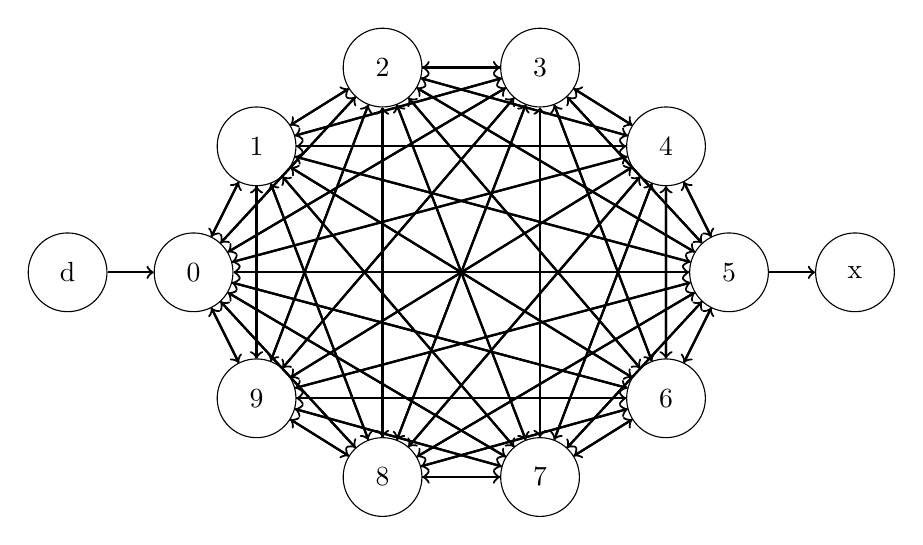
\begin{tikzpicture}[scale=0.2, every node/.style={draw=black,circle,inner sep=0pt}]
    \node [minimum size=1cm] (d) at (0,0) {d}; 
    \node [minimum size=1cm] (x) at (50,0) {x};                                    
    \node [minimum size=1cm] (0) at (8,0) {0};                                    
    \node [minimum size=1cm] (1) at (12,8) {1};                                    
    \node [minimum size=1cm] (2) at (20,13) {2};                                    
    \node [minimum size=1cm] (3) at (30,13) {3};                                    
    \node [minimum size=1cm] (4) at (38,8) {4};                                    
    \node [minimum size=1cm] (5) at (42,0) {5};                                    
    \node [minimum size=1cm] (6) at (38,-8) {6};                                    
    \node [minimum size=1cm] (7) at (30,-13) {7};                                    
    \node [minimum size=1cm] (8) at (20,-13) {8};                                    
    \node [minimum size=1cm] (9) at (12,-8) {9};                                    
    \draw [thick, ->] (d) -- (0);                                 
    \draw [thick, ->] (5) -- (x);                                 
    \draw [thick, ->] (0) -- (1);                                 
    \draw [thick, ->] (0) -- (2);                                 
    \draw [thick, ->] (0) -- (3);                                 
    \draw [thick, ->] (0) -- (4);                                 
    \draw [thick, ->] (0) -- (5);                                 
    \draw [thick, ->] (0) -- (6);                                 
    \draw [thick, ->] (0) -- (7);                                 
    \draw [thick, ->] (0) -- (8);                                 
    \draw [thick, ->] (0) -- (9);                                 
    \draw [thick, ->] (1) -- (0);                                 
    \draw [thick, ->] (1) -- (2);                                 
    \draw [thick, ->] (1) -- (3);                                 
    \draw [thick, ->] (1) -- (4);                                 
    \draw [thick, ->] (1) -- (5);                                 
    \draw [thick, ->] (1) -- (6);                                 
    \draw [thick, ->] (1) -- (7);                                 
    \draw [thick, ->] (1) -- (8);                                 
    \draw [thick, ->] (1) -- (9);                                 
    \draw [thick, ->] (2) -- (1);                                 
    \draw [thick, ->] (2) -- (0);                                 
    \draw [thick, ->] (2) -- (3);                                 
    \draw [thick, ->] (2) -- (4);                                 
    \draw [thick, ->] (2) -- (5);                                 
    \draw [thick, ->] (2) -- (6);                                 
    \draw [thick, ->] (2) -- (7);                                 
    \draw [thick, ->] (2) -- (8);                                 
    \draw [thick, ->] (2) -- (9);                                 
    \draw [thick, ->] (3) -- (1);                                 
    \draw [thick, ->] (3) -- (2);                                 
    \draw [thick, ->] (3) -- (0);                                 
    \draw [thick, ->] (3) -- (4);                                 
    \draw [thick, ->] (3) -- (5);                                 
    \draw [thick, ->] (3) -- (6);                                 
    \draw [thick, ->] (3) -- (7);                                 
    \draw [thick, ->] (3) -- (8);                                 
    \draw [thick, ->] (3) -- (9);                                 
    \draw [thick, ->] (4) -- (1);                                 
    \draw [thick, ->] (4) -- (2);                                 
    \draw [thick, ->] (4) -- (3);                                 
    \draw [thick, ->] (4) -- (0);                                 
    \draw [thick, ->] (4) -- (5);                                 
    \draw [thick, ->] (4) -- (6);                                 
    \draw [thick, ->] (4) -- (7);                                 
    \draw [thick, ->] (4) -- (8);                                 
    \draw [thick, ->] (4) -- (9);                                 
    \draw [thick, ->] (5) -- (1);                                 
    \draw [thick, ->] (5) -- (2);                                 
    \draw [thick, ->] (5) -- (3);                                 
    \draw [thick, ->] (5) -- (4);                                 
    \draw [thick, ->] (5) -- (0);                                 
    \draw [thick, ->] (5) -- (6);                                 
    \draw [thick, ->] (5) -- (7);                                 
    \draw [thick, ->] (5) -- (8);                                 
    \draw [thick, ->] (5) -- (9);                                 
    \draw [thick, ->] (6) -- (1);                                 
    \draw [thick, ->] (6) -- (2);                                 
    \draw [thick, ->] (6) -- (3);                                 
    \draw [thick, ->] (6) -- (4);                                 
    \draw [thick, ->] (6) -- (5);                                 
    \draw [thick, ->] (6) -- (0);                                 
    \draw [thick, ->] (6) -- (7);                                 
    \draw [thick, ->] (6) -- (8);                                 
    \draw [thick, ->] (6) -- (9);                                 
    \draw [thick, ->] (7) -- (1);                                 
    \draw [thick, ->] (7) -- (2);                                 
    \draw [thick, ->] (7) -- (3);                                 
    \draw [thick, ->] (7) -- (4);                                 
    \draw [thick, ->] (7) -- (5);                                 
    \draw [thick, ->] (7) -- (6);                                 
    \draw [thick, ->] (7) -- (0);                                 
    \draw [thick, ->] (7) -- (8);                                 
    \draw [thick, ->] (7) -- (9);                                 
    \draw [thick, ->] (8) -- (1);                                 
    \draw [thick, ->] (8) -- (2);                                 
    \draw [thick, ->] (8) -- (3);                                 
    \draw [thick, ->] (8) -- (4);                                 
    \draw [thick, ->] (8) -- (5);                                 
    \draw [thick, ->] (8) -- (6);                                 
    \draw [thick, ->] (8) -- (7);                                 
    \draw [thick, ->] (8) -- (0);                                 
    \draw [thick, ->] (8) -- (9);                                 
    \draw [thick, ->] (9) -- (1);                                 
    \draw [thick, ->] (9) -- (2);                                 
    \draw [thick, ->] (9) -- (3);                                 
    \draw [thick, ->] (9) -- (4);                                 
    \draw [thick, ->] (9) -- (5);                                 
    \draw [thick, ->] (9) -- (6);                                 
    \draw [thick, ->] (9) -- (7);                                 
    \draw [thick, ->] (9) -- (8);                                 
    \draw [thick, ->] (9) -- (0);                                 
\end{tikzpicture}                                                       

		 \caption{Clique graph example}
    	 \label{fig:clique_topology}
     \end{subfigure}
     \hfill
     \begin{subfigure}[b]{0.45\textwidth}
         \centering
         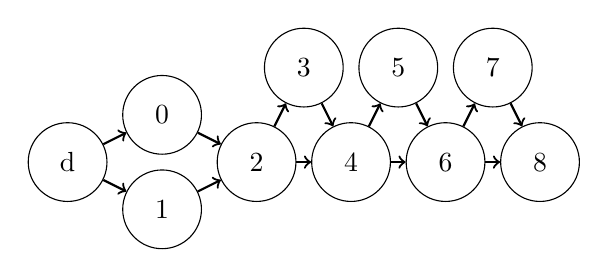
\begin{tikzpicture}[scale=0.15, every node/.style={draw=black,circle,inner sep=0pt}]
    \node [minimum size=1cm] (d) at (0,0) {d}; 
    \node [minimum size=1cm] (0) at (8,4) {0}; 
    \node [minimum size=1cm] (1) at (8,-4) {1}; 
    \node [minimum size=1cm] (2) at (16,0) {2}; 
    \node [minimum size=1cm] (3) at (20,8) {3}; 
    \node [minimum size=1cm] (4) at (24,0) {4}; 
    \node [minimum size=1cm] (5) at (28,8) {5}; 
    \node [minimum size=1cm] (6) at (32,0) {6}; 
    \node [minimum size=1cm] (7) at (36,8) {7}; 
    \node [minimum size=1cm] (8) at (40,0) {8}; 
    \draw [thick, ->] (d) -- (0);
    \draw [thick, ->] (d) -- (1);
    \draw [thick, ->] (0) -- (2);
    \draw [thick, ->] (1) -- (2);
    \draw [thick, ->] (2) -- (3);
    \draw [thick, ->] (2) -- (4);
    \draw [thick, ->] (3) -- (4);
    \draw [thick, ->] (4) -- (5);
    \draw [thick, ->] (4) -- (6);
    \draw [thick, ->] (5) -- (6);
    \draw [thick, ->] (6) -- (7);
    \draw [thick, ->] (6) -- (8);
    \draw [thick, ->] (7) -- (8);
\end{tikzpicture}                                                       


		 \caption{Fabrikant chain graph example}
		 \label{fig:fabrikant_topology}
     \end{subfigure}
		\caption{Simple topologies used in the thesis}
        \label{fig:clique_and_fabrikant}
\end{figure}

The last type of topology used points to resemble the properties of the actual
Internet graph.
It uses the property studied and described by Elmokashfi et al. in \cite{elmokashfi2010scalability}.
An example with few nodes is available in \cref{fig:internet_like_topology}.
The internet graph is actually a hierarchical graph clearly separated in multiple
levels by the type and properties of the nodes.

\begin{figure}[ht]
     \centering
     \begin{subfigure}[b]{0.49\textwidth}
         \centering
         \includegraphics[width=\textwidth]{images/internet_graph/graph-100-colored.pdf}
		 \caption{Internet like graph with an \q{explosive} layout}
         \label{fig:internet_topology_explosive}
     \end{subfigure}
     \hfill
     \begin{subfigure}[b]{0.49\textwidth}
         \centering
         \includegraphics[width=\textwidth]{images/internet_graph/graph_dot.pdf}
		 \caption{\q{Hierarchical} Internet like graph}
         \label{fig:internet_topology_hierarchical}
     \end{subfigure}
        \caption{Internet like graph coloured to show the hierarchical structure,
4 types of nodes, T (tier 1 mesh), M, CP, C (Customers, the purple one)}
        \label{fig:internet_like_topology}
\end{figure}

    \chapter{Discrete Event Simulator}
\label{cha:des}

Experiments on \ac{BGP} are not applicable on the Internet, for this
reason different studies shows their results using a simulate environment
\cite{griffin2001experimental} \fxfatal{Insert other citations}.
The majority of the studies uses small graphs, and each node 
of the graph simulate the behaviour of a \ac{BGP} speaker.
Each node represent also a single \ac{AS} and the \ac{BGP} speaker is it's own
exterior router, for simplicity reduced to one speaker that handles all the
connections.
 
For this reason I decided to use and expand a \ac{DES} that permits to have
different grades of freedom, respecting on the other side all the properties
required for a reliable simulator environment.
I decided to use the \textit{Simpy}\footnote{\href{https://simpy.readthedocs.io/en/latest/index.html}{Simpy website}}
package to make the environment evolve. I decided for this package for the
extensive documentation and because it has been already used for different
studies, demonstrating its adaptability \cite{matloff2008introduction,dagkakis2013manpy}.

I developed the \ac{DES} as a highly modular environment.
\begin{figure}[h]                                                               
    \begin{center}                                                              
        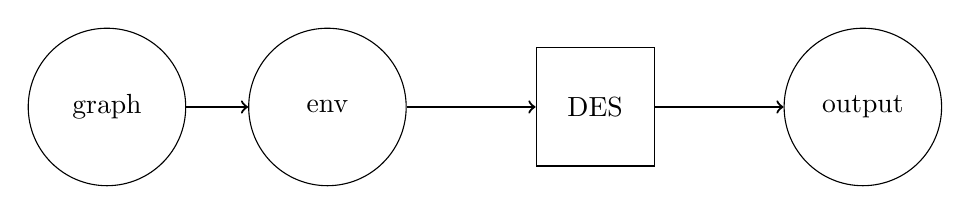
\begin{tikzpicture}[scale=0.2, every node/.style={draw=black,circle,inner sep=0pt}]
    \node [minimum size=2cm] (graph) at (0,0) {graph}; 
    \node [minimum size=2cm] (env) at (14,0) {env};                                    
    \node [rectangle, draw, minimum width=1.5cm,minimum height=1.5cm] (des) at (31,0) {DES};
    \node [minimum size=2cm] (output) at (48,0) {output};                                    
    \draw [thick, ->] (graph) to (env);                                  
    \draw [thick, ->] (env) -- (des);                                 
    \draw [thick, ->] (des) -- (output);                                 
\end{tikzpicture}                                                       

    \end{center}                                                                
    \caption{Discrete event simulator structure}                                
    \label{fig:des_structure}                                                   
\end{figure}
In \Cref{fig:des_structure} is possible to see the basic idea of the simulator.
The first component needed is a graph, represented by a \textit{graphml} file, this file is 
descriptor of the network. it defines also all topological information and all the
properties of each single node.
\fxfatal{Look for a Cref implementation of this}
In Code \ref{lst:graph_example} is possible to see an example of a \textit{graphml} file,
it describes that node \num{0} contains a single destination and that the edge
between nodes \num{2} and \num{5} is controlled by the policy |2, 2, 2| that defines
a servicer-provider policy.
Policies are encoded using the convention described in \cite{daggitt2018rate}.

\lstcaptionname{Code}
\begin{lstlisting}[language=graphml, caption=Graph example, label=lst:graph_example]
 <node id="0">
      <data key="d0">10.0.0.0/24</data>
 </node>
 <edge source="2" target="5">                                                  
     <data key="d2">2, 2, 2</data>                                             
 </edge> 
\end{lstlisting}

The graph is then embedded in the environment file, this file is in \textit{json}
format and it describes how the environment is characterized, it gives the
initial values for the \ac{RNG} so that each experiment is replicable and
other properties, like where the output should be saved, and, most importantly
how the experiment should be conducted.
There are two possible evolution of the environment:
\begin{itemize}
    \item \textbf{\textit{Continuous evolution}}: In this category all the nodes
    that contains at least a destination will continuously share and retrieve
    the destination accordingly with the distributions defined in the environment;
    \item \textbf{\textit{Signaling evolution}}: Is possible to define a precise
    signal that should be executed by the nodes that contains a destination, for 
    example, the signal \q{AWA} defines that there will be an announce followed by 
    a withdraw and the an other announce.
\end{itemize}

The \ac{DES} take as input this \textit{json} file where all the information
are described, it creates an object for each node in the graph file, with
each own characteristics.
After the initialization all the nodes that contains a destination will schedule
the first advertisement of it to their neighbour.
The simulation run will terminate only if there are no more events scheduled or
if the maximum simulation time is reached.

The \ac{DES} will then produce a \textit{CSV} output, with all the events that 
can be analyzed to see the evolution of a specific node or to evaluate the
whole network.
 
\section{DES Environments}
\label{sec:des_environment}

\begin{itemize}
    \item Example environment
    \item Explanation of more complex environments
    \item Internet like graphs
    \item Fabrikant Graphs
\end{itemize}

Thanks to the environment codification in a \textit{json} file is possible to
define experiments with a high grade of freedom.
Is possible to define multiple delays as probability functions vectors that
will provide multiple runs possibility. For example, if we have \num{5} different
possible seeds and \num{3} different delays, the total number of runs combinations
is \num{15}, as showed in Code \ref{lst:environment_example}.
is possible to run one of the possible combination of parameters through the identifier
of the single run.

\lstcaptionname{Code}
\begin{lstlisting}[language=json, caption=Environment example, label=lst:environment_example]
"simulation" : {                                                              
    // seed(s) to initialize RNG                                      
    "seed" : [0, 1, 2, 3, 4], 
    ....
    // Multiple withdraw distributions
    "withdraw_dist": [{"distribution": "unif", "min": 5, "max": 10, "int": 0.1},
                      {"distribution": "unif", "min": 8, "max": 10, "int": 0.1},
                      {"distribution": "unif", "min": 2, "max": 3, "int": 0.1}],       
    ....
}
\end{lstlisting}

In the environment is possible to define also the processing time, this time is used
inside each \ac{BGP} node to emulate the processing of information or the evaluation
of a packet.
Though the \textit{delay} parameter is possible to define the default delay on the edges,
is important to remember that the links are FIFO so there is no reordering
of messages in the same link, there is also no messages lost.
That because it was out of the scope of this thesis to study the evolution
of the protocol with packet loss, but it could be a future work.

\subsection{Clique environment}
\label{subsec:clique_env}

One of the special environment that I used it's composed by a clique graph
graph of different dimensions, an example of clique graph is given in
\Cref{fig:clique_graph}.

\begin{figure}[h]                                                               
    \begin{center}                                                              
        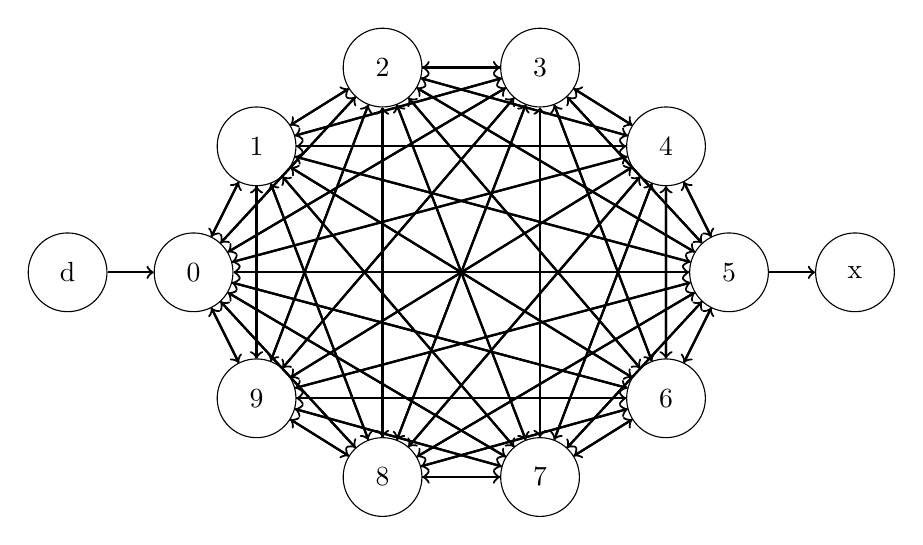
\begin{tikzpicture}[scale=0.2, every node/.style={draw=black,circle,inner sep=0pt}]
    \node [minimum size=1cm] (d) at (0,0) {d}; 
    \node [minimum size=1cm] (x) at (50,0) {x};                                    
    \node [minimum size=1cm] (0) at (8,0) {0};                                    
    \node [minimum size=1cm] (1) at (12,8) {1};                                    
    \node [minimum size=1cm] (2) at (20,13) {2};                                    
    \node [minimum size=1cm] (3) at (30,13) {3};                                    
    \node [minimum size=1cm] (4) at (38,8) {4};                                    
    \node [minimum size=1cm] (5) at (42,0) {5};                                    
    \node [minimum size=1cm] (6) at (38,-8) {6};                                    
    \node [minimum size=1cm] (7) at (30,-13) {7};                                    
    \node [minimum size=1cm] (8) at (20,-13) {8};                                    
    \node [minimum size=1cm] (9) at (12,-8) {9};                                    
    \draw [thick, ->] (d) -- (0);                                 
    \draw [thick, ->] (5) -- (x);                                 
    \draw [thick, ->] (0) -- (1);                                 
    \draw [thick, ->] (0) -- (2);                                 
    \draw [thick, ->] (0) -- (3);                                 
    \draw [thick, ->] (0) -- (4);                                 
    \draw [thick, ->] (0) -- (5);                                 
    \draw [thick, ->] (0) -- (6);                                 
    \draw [thick, ->] (0) -- (7);                                 
    \draw [thick, ->] (0) -- (8);                                 
    \draw [thick, ->] (0) -- (9);                                 
    \draw [thick, ->] (1) -- (0);                                 
    \draw [thick, ->] (1) -- (2);                                 
    \draw [thick, ->] (1) -- (3);                                 
    \draw [thick, ->] (1) -- (4);                                 
    \draw [thick, ->] (1) -- (5);                                 
    \draw [thick, ->] (1) -- (6);                                 
    \draw [thick, ->] (1) -- (7);                                 
    \draw [thick, ->] (1) -- (8);                                 
    \draw [thick, ->] (1) -- (9);                                 
    \draw [thick, ->] (2) -- (1);                                 
    \draw [thick, ->] (2) -- (0);                                 
    \draw [thick, ->] (2) -- (3);                                 
    \draw [thick, ->] (2) -- (4);                                 
    \draw [thick, ->] (2) -- (5);                                 
    \draw [thick, ->] (2) -- (6);                                 
    \draw [thick, ->] (2) -- (7);                                 
    \draw [thick, ->] (2) -- (8);                                 
    \draw [thick, ->] (2) -- (9);                                 
    \draw [thick, ->] (3) -- (1);                                 
    \draw [thick, ->] (3) -- (2);                                 
    \draw [thick, ->] (3) -- (0);                                 
    \draw [thick, ->] (3) -- (4);                                 
    \draw [thick, ->] (3) -- (5);                                 
    \draw [thick, ->] (3) -- (6);                                 
    \draw [thick, ->] (3) -- (7);                                 
    \draw [thick, ->] (3) -- (8);                                 
    \draw [thick, ->] (3) -- (9);                                 
    \draw [thick, ->] (4) -- (1);                                 
    \draw [thick, ->] (4) -- (2);                                 
    \draw [thick, ->] (4) -- (3);                                 
    \draw [thick, ->] (4) -- (0);                                 
    \draw [thick, ->] (4) -- (5);                                 
    \draw [thick, ->] (4) -- (6);                                 
    \draw [thick, ->] (4) -- (7);                                 
    \draw [thick, ->] (4) -- (8);                                 
    \draw [thick, ->] (4) -- (9);                                 
    \draw [thick, ->] (5) -- (1);                                 
    \draw [thick, ->] (5) -- (2);                                 
    \draw [thick, ->] (5) -- (3);                                 
    \draw [thick, ->] (5) -- (4);                                 
    \draw [thick, ->] (5) -- (0);                                 
    \draw [thick, ->] (5) -- (6);                                 
    \draw [thick, ->] (5) -- (7);                                 
    \draw [thick, ->] (5) -- (8);                                 
    \draw [thick, ->] (5) -- (9);                                 
    \draw [thick, ->] (6) -- (1);                                 
    \draw [thick, ->] (6) -- (2);                                 
    \draw [thick, ->] (6) -- (3);                                 
    \draw [thick, ->] (6) -- (4);                                 
    \draw [thick, ->] (6) -- (5);                                 
    \draw [thick, ->] (6) -- (0);                                 
    \draw [thick, ->] (6) -- (7);                                 
    \draw [thick, ->] (6) -- (8);                                 
    \draw [thick, ->] (6) -- (9);                                 
    \draw [thick, ->] (7) -- (1);                                 
    \draw [thick, ->] (7) -- (2);                                 
    \draw [thick, ->] (7) -- (3);                                 
    \draw [thick, ->] (7) -- (4);                                 
    \draw [thick, ->] (7) -- (5);                                 
    \draw [thick, ->] (7) -- (6);                                 
    \draw [thick, ->] (7) -- (0);                                 
    \draw [thick, ->] (7) -- (8);                                 
    \draw [thick, ->] (7) -- (9);                                 
    \draw [thick, ->] (8) -- (1);                                 
    \draw [thick, ->] (8) -- (2);                                 
    \draw [thick, ->] (8) -- (3);                                 
    \draw [thick, ->] (8) -- (4);                                 
    \draw [thick, ->] (8) -- (5);                                 
    \draw [thick, ->] (8) -- (6);                                 
    \draw [thick, ->] (8) -- (7);                                 
    \draw [thick, ->] (8) -- (0);                                 
    \draw [thick, ->] (8) -- (9);                                 
    \draw [thick, ->] (9) -- (1);                                 
    \draw [thick, ->] (9) -- (2);                                 
    \draw [thick, ->] (9) -- (3);                                 
    \draw [thick, ->] (9) -- (4);                                 
    \draw [thick, ->] (9) -- (5);                                 
    \draw [thick, ->] (9) -- (6);                                 
    \draw [thick, ->] (9) -- (7);                                 
    \draw [thick, ->] (9) -- (8);                                 
    \draw [thick, ->] (9) -- (0);                                 
\end{tikzpicture}                                                       

    \end{center}                                                                
    \caption{Clique graph example}                                
    \label{fig:clique_graph}
\end{figure}

The only node that shares a destination is the node \q{\textit{d}}, the node
\num{0} will then spread the knowledge to the whole network, and the node 
\q{\textit{x}} will act as a black hole for all the possible paths
that the node \num{5} will share.
This topology is used to enforce the path exploration problem.

\subsection{Fabrikant environment}
\label{subsec:fabrikant_env}

Another interesting chase to test the path exploration problem is the one
presented in \cite{fabrikant2011there}.
In that study Fabrikant et al. presents how particular \ac{MRAI} setting could 
make the network converge with an exponential bechaviour because of the path
exploration problem.
I used the basic example of their study to investigate how the choose of \ac{MRAI}
is foundamental for the network convergence.
An example of the network used is presented 
in \Cref{fig:fabrikant_graph}.

\begin{figure}[h]                                                               
    \begin{center}                                                              
        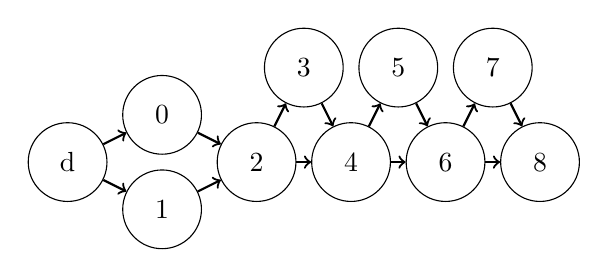
\begin{tikzpicture}[scale=0.15, every node/.style={draw=black,circle,inner sep=0pt}]
    \node [minimum size=1cm] (d) at (0,0) {d}; 
    \node [minimum size=1cm] (0) at (8,4) {0}; 
    \node [minimum size=1cm] (1) at (8,-4) {1}; 
    \node [minimum size=1cm] (2) at (16,0) {2}; 
    \node [minimum size=1cm] (3) at (20,8) {3}; 
    \node [minimum size=1cm] (4) at (24,0) {4}; 
    \node [minimum size=1cm] (5) at (28,8) {5}; 
    \node [minimum size=1cm] (6) at (32,0) {6}; 
    \node [minimum size=1cm] (7) at (36,8) {7}; 
    \node [minimum size=1cm] (8) at (40,0) {8}; 
    \draw [thick, ->] (d) -- (0);
    \draw [thick, ->] (d) -- (1);
    \draw [thick, ->] (0) -- (2);
    \draw [thick, ->] (1) -- (2);
    \draw [thick, ->] (2) -- (3);
    \draw [thick, ->] (2) -- (4);
    \draw [thick, ->] (3) -- (4);
    \draw [thick, ->] (4) -- (5);
    \draw [thick, ->] (4) -- (6);
    \draw [thick, ->] (5) -- (6);
    \draw [thick, ->] (6) -- (7);
    \draw [thick, ->] (6) -- (8);
    \draw [thick, ->] (7) -- (8);
\end{tikzpicture}                                                       


    \end{center}                                                                
    \caption{Fabrikant chain graph example}                                
    \label{fig:fabrikant_graph}
\end{figure}

The path exploration problem is caused by the delay on the node \num{0}-\num{2}
edge. The node 2 will receive the destination through node 1, after a small ammount
of time the network will converge to the best path (without using the backup links).
But, after a while, node \num{2} will receive the network also through node \num{0}
and it will prefer this new path, provoking then the riconfiguration of all
the other nodes that will use the backup links for a while, announcing their 
new path.
A wrong configuration of \ac{MRAI} can provoke the entire exploration of the 
possibility set.

\subsection{Internet-like environment}
\label{subsec:internet_like_env}

The last noteworthy environment is the one whose purpose is to simulate Internet
behaviour.
This has been possible thanks to the study by Elmokashfi et al. \cite{elmokashfi2010scalability}
and the internet like graph generator present in Networkx\footnote{\href{https://networkx.org/documentation/stable/reference/generated/networkx.generators.internet_as_graphs.random_internet_as_graph.html#networkx.generators.internet_as_graphs.random_internet_as_graph}{Networkx internet as graph generator}}
(a python library famous for graph and network studies).
An example with a small set of nodes is presented in \Cref{fig:internet_graphs}

\begin{figure}[h]
     \centering
     \begin{subfigure}[b]{0.45\textwidth}
         \centering
         \includegraphics[width=\textwidth]{images/internet_graph/graph-100-colored.pdf}
		 \caption{Internet like graph with an \q{explosive} layout}
         \label{fig:internet_graph_explosive}
     \end{subfigure}
     \hfill
     \begin{subfigure}[b]{0.45\textwidth}
         \centering
         \includegraphics[width=\textwidth]{images/internet_graph/graph_dot.pdf}
		 \caption{Internet like graph with a \q{hierarchical} layout}
         \label{fig:internet_graph_hierarchical}
     \end{subfigure}
        \caption{Internet like graph colored to show the hierarchicaly structure,
4 tipes of nodes, T (tier 1 mesh), M, CP, C (Customers, purple one)}
        \label{fig:internet_graphs}
\end{figure}

The different nodes are colored accordingly with the node type represented.
The tier one nodes that generate the centrali clique are colored in red, and
is possible to notice in \Cref{fig:internet_graph_hierarchical} that them are
in the highest levels of the networks.
This environment has been used to study the behaviour of the network with 
topologies resempbling the real internet.

    \chapter{The Protocol as a Finite State Machine}
\label{cha:bgp_fsm}

The incremental nature of \ac{BGP} suggests that is possible to study the
evolution of the protocol looking to the events that has been triggered
and the causes of them.
A model that can give this sort of information would be helpful to debug 
the protocol, analyze faulty situations or prevent them.
The main idea behind this model of the protocol has been taken and 
expanded from \cite{griffinFSM}.
I'm going to show that infering information from \ac{BGP} events and actions
is more difficult than what expected.
In fact, due to the \textit{Path Exploration} problem, presented in \Cref{sec:bgp_fsm_explosion},
the node will experience an explosion in the number of possible evolutions.
Multiple inputs can lead to the same output of the node, so its not enough to
know it to infer a precise input signal.
Furthermore, \ac{MRAI} can make the situation even more complicated, increasing
the number of transitions.

\section{BGP generalization}
\label{sec:bgp_generalization}

The main idea behind the \ac{BGP} \ac{FSM} is to represent the knowledge as
states and different set of messages as transitions.
The knowledge is represented by the actual routes that the node knows on how 
to reach a single destination.
Transitions encode the messages that a node has received to trigger the state change,
on the edges are also inserted the response messages that the node will transmit.
We can see an example of this transitions in \Cref{fig:fsm_example}

\begin{figure}[h]                                                               
    \begin{center}                                                              
        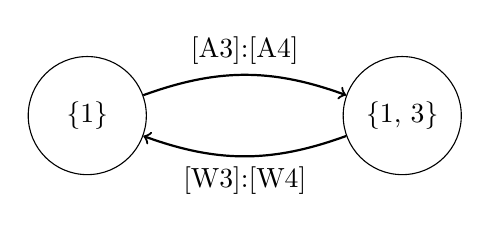
\begin{tikzpicture}[scale=0.2, state/.style={draw=black,circle,inner sep=0pt}]
	\node [state, minimum size=1.5cm] (s1) at (0,0) {\{1\}}; 
	\node [state, minimum size=1.5cm] (s2) at (20,0) {\{1, 3\}};
	%\draw[arrow](B1.west) to [out=190,in=170] node[above]{Flow: $\alpha$ } (S1.west);
	\draw [thick, ->] (s1) to[out=20, in=160] node[above]{[\q{A3}]:[\q{A4}]} (s2); 
	\draw [thick, ->] (s2) to[out=-160, in=-20] node[below]{[\q{W3}]:[\q{W4}]} (s1);
\end{tikzpicture}                        

    \end{center}                                                                
	\caption{Example of the \ac{BGP} \ac{FSM} state transition}
    \label{fig:fsm_example}                                                   
\end{figure}

In \Cref{fig:fsm_example} there are two states, both represent the knowledge of
the node, the first one represent the \ac{RIB} with just the route \num{1}, in
the second state the \ac{RIB} will contains both the routes \num{1} and \num{3}.
This transition si caused by the reception of the advertisement of the route 
\num{3} and will couse the transmission of an other advertisement.
The opposite transition is caused by the reception of the withdraw of the route
\num{4} with the consequent withdraw of the route \num{4}.

In \ac{BGP} messages transfer information about routes, there could be the advertisement
or the withdraw of the route.

Thanks to \ac{MRAI} the evaluation of multiple messages could be delayed and
provoke then the compression of them.
For this reason on the edges is possible to see multiple messages, for example 
\q{A1W1A1}, that will be compressed in \q{A1} and then evaluated.

The concept for a \ac{BGP} \ac{FSM} has been expanded from \cite{griffinFSM}.

%\begin{itemize}
%    \item BGP as an FSM main idea
%    \item signalling transmutation
%\end{itemize}

\section{BGP FSM experiments}
\label{sec:bgp_fsm_experiments}

The first experiments, about the translation of a single node evolution in a
\ac{FSM}, goal is to reproduce what has been shown in \cite{griffinFSM}.
The graph used for the study is presented in \cref{fig:griffin_fig_4}.

\begin{figure}[h]                                                               
    \begin{center}                                                              
        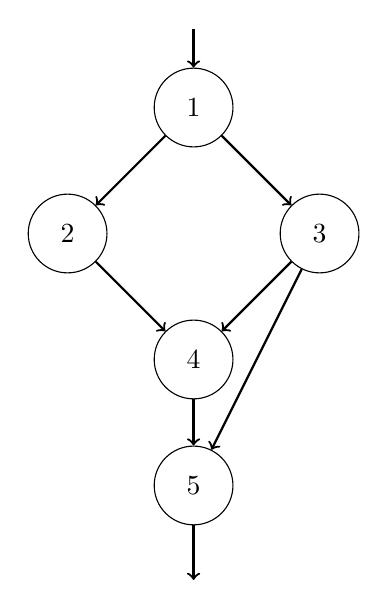
\begin{tikzpicture}[scale=0.2, every node/.style={draw=black,circle,inner sep=0pt}]
    \node [minimum size=1cm] (1) at (0,0) {1}; 
    \node [minimum size=1cm] (2) at (-8,-8) {2}; 
    \node [minimum size=1cm] (3) at (8,-8) {3}; 
    \node [minimum size=1cm] (4) at (0,-16) {4}; 
    \node [minimum size=1cm] (5) at (0,-24) {5}; 
	\draw [thick, ->] (0, 5) -- (1);
    \draw [thick, ->] (1) -- (2);
    \draw [thick, ->] (1) -- (3);
    \draw [thick, ->] (2) -- (4);
    \draw [thick, ->] (3) -- (4);
    \draw [thick, ->] (3) -- (5);
    \draw [thick, ->] (4) -- (5);
	\draw [thick, ->] (5) -- (0, -30);
\end{tikzpicture}                                                       


    \end{center}                                                                
	\caption{Graph from fig 4 of \cite{griffinFSM} used to study the \ac{FSM}
		of the nodes}                                
    \label{fig:griffin_fig_4}                                                   
\end{figure}

This topology, \Cref{fig:griffin_fig_4}, present an \ac{SPP} with five nodes \cite{griffin2002stable}. 
The \ac{SPP} model is used to eliminate much of the complexity of \ac{BGP}.
The arrows in the graph represent the flow of information, node \num{1} is the one
that will receive a new route to reach a hypothetical destination and it will 
spread this information through an \ac{ADV} to all it neighbours.
The translation to the \ac{CFSM} will use an enumeration to encode all the
paths that a single node will encounter, for example, the path \q{5 3 1} will
be converted in \textit{a3}, each path has its own identifier.
In case of withdraw the route will be encoded as \textit{w3}.

The properties of the environment for this experiment are listed in \Cref{tbl:fig_4_example}.

\begin{table}[h]
	\begin{center}
	\begin{tabular}{ || m{4cm}| m{7.5cm} || }
	\hline
	Property & Value \\
	\hline \hline
	Seeds & $[1, 50]$ \\
	\hline
	Signaling & \q{AW} \\
	\hline
	Withdraws delay & Uniform distribution between \SI{20}{\second} and \SI{30}{\second} \\
	\hline
	Announcement delay & Uniform distribution between \SI{20}{\second} and \SI{30}{\second} \\
	\hline
    \ac{MRAI} & \SI{0}{\second} for every link \\
	\hline
	Link delay & Uniform distribution between \SI{0.001}{\second} adn \SI{1}{\second}, uniform distribution between \SI{0.012}{\second} and \SI{3}{\second} \\
	\hline
    \ac{IW} & Active \\
	\hline
	\end{tabular}
\end{center}

	\caption{FSM example environment properties}
	\label{tbl:fig_4_example}
\end{table}

The total number of runs generated by this environment is \num{100}.

\fxfatal{this paragraph is cumbersome}
The two nodes of more interest are node \num{4} and node \num{4}.
The first one can receive multiple combinations of messages from node \num{2} and
\num{3}, for sure there will be two announcements and two withdraws because node
1 has to respect a predefined signaling. but, those messages could be reordered
in different ways, and, for each sequence of them we can encounter a different
sequence of output messages through node \num{5}.
Giving that the routes from node \num{2} and \num{3} will have respectively as 
ID \num{2}, \num{3} the table \Cref{tbl:fig_4_node4_possible_inputs}
All possible inputs of node \num{4} are the shuffle of all possible
outputs of nodes \num{2} and \num{3} preserving the local order.

\begin{table}[h]
	\begin{center}
	\begin{tabular}{ || m{3cm}| m{3cm} || }
	\hline
	Input signal & Output signal\\
	\hline \hline
	$a2a3w2w3$ & $a4a5w4$ \\
	$a2a3w3w2$ & $a4w4$ \\
	$a3a2w2w3$ & $a5a4a5w5$ \\
	$a3a2w3w2$ & $a5a4w4$ \\
	$a2w2a3w3$ & $a4w4a5w5$ \\
	$a3w3a2w2$ & $a5w5a4w4$ \\
	\hline
	\end{tabular}
\end{center}


	\caption{Node 4 different possible inputs and output}
	\label{tbl:fig_4_node4_possible_inputs}
\end{table}

The node \num{5} will receive all the possible outputs from node \num{3} and 
\num{4} increasing the number of possible signals from \num{6} of node \num{4}
up to \num{71} but some of them produce the same output signal, so we have in 
total \num{52} unique output signals from node \num{5}.

From the \num{100} total runs we can generate the \ac{CFSM} of node \num{4} and
node \num{5}, in order to be able to study how the nodes reacts to different
input signals.
The two \ac{CFSM} are presented in \Cref{fig:fsm_griffin_fig4}.

\fxfatal{Remove message table from \Cref{fig:fsm_griffin_fig4}?}
\begin{figure}[h]
     \centering
     \begin{subfigure}[b]{0.45\textwidth}
         \centering
         \includegraphics[width=\textwidth]{images/fsm/fig_4_4.pdf}
		 \caption{Node \num{4} \ac{CFSM} from the environment of \Cref{tbl:fig_4_example}}
         \label{fig:fsm_node4}
     \end{subfigure}
     \hfill
     \begin{subfigure}[b]{0.45\textwidth}
         \centering
         \includegraphics[width=\textwidth]{images/fsm/fig_4_5.pdf}
		 \caption{Node \num{5} \ac{CFSM} from the environment of \Cref{tbl:fig_4_example}}
         \label{fig:fsm_node5}
     \end{subfigure}
		\caption{\ac{CFSM} of nodes \num{4} and \num{5} of the graph \Cref{fig:griffin_fig_4} with an input signal of \q{AW}}
        \label{fig:fsm_griffin_fig4}
\end{figure}

The states of the \ac{CFSM} in \Cref{fig:fsm_griffin_fig4} are represented by the
knowledge of the nodes, composed by the routes that are in the \ac{RIB} of the node.
The bold value is the actual best route to the destination chosen by the node.
If in the state transition to a new state the best path is not affected then the
node will not transmit the new route to its neighbours, for an example take
a look to \Cref{fig:fsm_node4} from the state $\{1\}$ to the state $\{1, 3\}$
where the node \num{4} will learn a new route that is not the best one.

The effects of the implicit withdraw can be seen in \Cref{fig:fsm_node5}
the transition from $\{1, 4\}$ to $\{1, 3\}$ thanks to the reception of the
announcement $a3$ from the node \num{4}.

As written in \cite{griffinFSM}, I would like to underline the fact that, given
the \num{52} unique possible outputs of the node \num{5} it would be very difficult
to infer the initial signal that provokes all the transitions.

We can also analyze those output signals, having all the events for each single
run we can infer which were the most common output signals that a single node
experienced.
Is sufficient to take all the transmitted messages of a node and look the sequence
of advertisement and withdraws.

\begin{figure}[h]
     \centering
     \begin{subfigure}[b]{0.45\textwidth}
         \centering
         \includegraphics[width=\textwidth]{images/signal_study/fig_4/fig_4_4_signaling_nmessage_prob.pdf}
		 \caption{Node \num{4} output signals study}
         \label{fig:signal_node4}
     \end{subfigure}
     \hfill
     \begin{subfigure}[b]{0.45\textwidth}
         \centering
         \includegraphics[width=\textwidth]{images/signal_study/fig_4/fig_4_5_signaling_nmessage_prob.pdf}
		 \caption{Node \num{5} output signals study}
         \label{fig:signal_node5}
     \end{subfigure}
		\caption{Output signal study of nodes \num{4} and \num{5} of the graph 
			\Cref{fig:griffin_fig_4} with an input signal of \q{AW} at node \num{1}}
        \label{fig:signal_griffin_fig4}
\end{figure}

The plots in \Cref{fig:signal_griffin_fig4} represents the probability of an
output signal of a certain length to appear and the number of unique output signals
of a unique length has been found.
The $x$ axis represents the number of messages in the output signal, a message
is a single announcement or withdraw.
The first $y$ axis represents the probability to see a certain number of messages
taking a random output signal from the output.
For this axis there are three lines that refer to it, the blue one represent the
number of advertisement messages in the output signal correlated with the 
respective probability.
For example, in \Cref{fig:signal_node4} there is a probability around $0.45$ to have
exactly two advertisement messages per output signal. And respectively a probability
slightly larger than $0.25$ to have only one advertisement or three.
We can also notice that we didn't see more than three advertisements or less than one.
The green line instead represents the total number of messages in the signal,
without distinguishing between advertisement and withdraws.
By the fact that we will always have one withdraw (the orange line) this line 
is simply shifted by one unit in respect of the advertisement line.
The second $y$ axis refers to the number of unique output signals encountered and
their length.
For example, in \Cref{fig:signal_node5} we will have \num{1} unique output signal
of length \num{2}, \num{3} signals of length \num{3} and \num{4} of length \num{4} and \num{2} of length \num{5}.

Those plots do not give a complete prospective of all the possible outputs
that can be generated but only the ones encountered during the runs.
In fact, during the \num{100} runs we encountered only the output signals listed
in \cref{tbl:signals}.

\begin{table}[h]
	\begin{subtable}[h]{0.45\textwidth}
		\begin{center}
	\begin{tabular}{ || m{3cm}| m{3cm} || } 
	\hline
	Signal & Frequency\\ 
	\hline \hline
		$a1a2a1w1$ & \num{28} \\
		$a2a1w1$ & \num{23} \\
		$a2w2$ & \num{26} \\
		$a1a2w2$ & \num{23} \\
	\hline
	\end{tabular}
\end{center}


		\caption{Node \num{4} output signals encountered}
		\label{tab:node4_outSignals}
    \end{subtable}
	\hfill
	\begin{subtable}[h]{0.45\textwidth}
		\begin{center}
	\begin{tabular}{ || m{3cm}| m{3cm} || } 
	\hline
	Signal & Frequency\\ 
	\hline \hline
	$a1a2a3w3$ & \num{15}\\
	$a1a3w3$ & \num{16}\\
	$a2a1a2w2$ & \num{19}\\
	$a1a2w2$ & \num{28}\\
	$a1w1$ & \num{2}\\
	$a2a1a3w3$ & \num{6}\\
	$a2a1a2a3w3$ & \num{8}\\
	$a3a1a2a3w3$ & \num{3}\\
	$a2a1w1$ & \num{2}\\
	$a3a1a3w3$ & \num{1}\\
	\hline
	\end{tabular}
\end{center}


		\caption{Node \num{5} output signals encountered}
		\label{tab:node5_outSignals}
    \end{subtable}
	\caption{Node 4 and 5 different output signals encountered during the runs}
	\label{tbl:signals}
\end{table}


\subsection{MRAI and BGP FSM}
\label{subsec:mrai_vs_bgpfsm}

How would \ac{MRAI} affect the study of the signals produced by \Cref{fig:griffin_fig_4}?
The answer is that the number of states will be the same but the number of possible
transitions will explode because there will be a lot more possible
input signals that will be compressed and evaluated by the nodes.

We can see the effects of \ac{MRAI} on the \ac{CFSM}s in \Cref{fig:fsm_griffin_fig4_MRAI}.

\fxfatal{\Cref{fig:fsm_node5_MRAI} is not readable at all, move the two figure
	one after the other}
\begin{figure}[h]
     \centering
     \begin{subfigure}[b]{0.45\textwidth}
         \centering
         \includegraphics[width=\textwidth]{images/fsm/fig_4_4_MRAI30.pdf}
		 \caption{Node \num{4} \ac{CFSM} from the environment of \Cref{tbl:fig_4_example} with \ac{MRAI}=\SI{30}{\second}}
         \label{fig:fsm_node4_MRAI}
     \end{subfigure}
     \hfill
     \begin{subfigure}[b]{0.45\textwidth}
         \centering
         \includegraphics[width=\textwidth]{images/fsm/fig_4_5_MRAI30.pdf}
		 \caption{Node \num{5} \ac{CFSM} from the environment of \Cref{tbl:fig_4_example} with \ac{MRAI}=\SI{30}{\second}}
         \label{fig:fsm_node5_MRAI}
     \end{subfigure}
		\caption{\ac{CFSM} of nodes \num{4} and \num{5} of the graph 
			\Cref{fig:griffin_fig_4} with an input signal of \q{AW} with
			\ac{MRAI}=\SI{30}{\second}}
        \label{fig:fsm_griffin_fig4_MRAI}
\end{figure}

\Cref{fig:fsm_node4} and \Cref{fig:fsm_node4_MRAI} permits us to compare the two
\ac{CFSM}s of node \num{4} and is possible to nice a big difference in terms of edges
between one figure and the other, the first one has \num{8} transitions, the
second one \num{15}.
For the node \num{5} we pass from \num{16} transitions to \num{36}.

But the positive effects of \ac{MRAI} can be found in the output signals, 
showed in \Cref{fig:signal_griffin_fig4_MRAI}.

\begin{figure}[h]
     \centering
     \begin{subfigure}[b]{0.45\textwidth}
         \centering
         \includegraphics[width=\textwidth]{images/signal_study/fig_4_MRAI/fig_4_4_signaling_nmessage_prob.pdf}
		 \caption{Node \num{4} output signals study with \ac{MRAI}=\SI{30}{\second}}
         \label{fig:signal_node4_MRAI}
     \end{subfigure}
     \hfill
     \begin{subfigure}[b]{0.45\textwidth}
         \centering
         \includegraphics[width=\textwidth]{images/signal_study/fig_4_MRAI/fig_4_5_signaling_nmessage_prob.pdf}
		 \caption{Node \num{5} output signals study with \ac{MRAI}=\SI{30}{\second}}
         \label{fig:signal_node5_MRAI}
     \end{subfigure}
		\caption{Output signal study of nodes \num{4} and \num{5} of the graph 
			\Cref{fig:griffin_fig_4} with an input signal of \q{AW} at node \num{1}
			with \ac{MRAI}=\SI{30}{\second} for every link}
        \label{fig:signal_griffin_fig4_MRAI}
\end{figure}

Comparing \Cref{fig:signal_node5_MRAI,fig:signal_node5} is possible to notice
that there is a different distribution of output signals.
The $x$ axis never reach the value of \num{5}, this means that the output signals
of the node \num{5} never used more than \num{4} messages.
And we can also notice that the majority of the signals this time have a length
of \num{3} messages, instead of the previous \num{4}.
This is a hint that \ac{MRAI} can have positive effects on the number of output messages
produced by single nodes, having, however, more possible transitions to consider.

\section{BGP FSM explosion}
\label{sec:bgp_fsm_explosion}

We know that \ac{MRAI} is not an easy parameter, the incorrect setting of
it can lead to an explosion of messages and an exponential convergence time.
This problem has been studied by Fabrikant et al. \cite{fabrikant2011there} and
the origin of the problem has been attributed to the \textit{path exploration}
problem.
This is a well-known problem in the \ac{BGP} community and it is experienced
by a node when it enters in a transitory phase where it accepts and publishes not
optimal paths towards the destination before reaching a stable state.
\textit{Path exploration} can lead to an enormous amount of messages even with
a small set of nodes \cite{deshpande2004impact}.

As we saw in \Cref{subsec:mrai_vs_bgpfsm} that \ac{MRAI} can influence the
\ac{CFSM}s of the nodes and their output signals, which impact could it have
if it is not set correctly?

I have then created an environment that resembles the study conducted by
\cite{fabrikant2011there} using a topology like the one described in \Cref{subsec:fabrikant_env}
with \num{3} rings.
with different \ac{MRAI} settings.
The environment properties are presented in \Cref{tbl:fabrikant_environment}.

\begin{table}[h]
	\begin{center}
	\begin{tabular}{ || m{4cm}| m{7.5cm} || }
	\hline
	Property & Value \\
	\hline \hline
	Seeds & $[1, 30]$ \\
	\hline
		Signaling & \q{A}, \q{AW}, \q{AWA}, \q{AWAW} \\
	\hline
		Withdraws delay & Uniform distribution between \SI{5}{\second} and \SI{10}{\second}, Uniform distribution between \SI{10}{\second} and \SI{15}{\second} \\
	\hline
	Announcement delay & Uniform distribution between \SI{5}{\second} and \SI{10}{\second}, Uniform distribution between \SI{10}{\second} and \SI{15}{\second} \\
	\hline
	Link delay & Uniform distribution between \SI{0.5}{\second} adn \SI{3}{\second}, uniform distribution between \SI{2}{\second} and \SI{4}{\second} \\
	\hline
	\end{tabular}
\end{center}

	\caption{Fabrikant experiments environment}
	\label{tbl:fabrikant_environment}
\end{table}

In total, for each signaling experiment this environment produces \num{240} runs.
I have then introduced \num{4} different \ac{MRAI} strategies for each different
signal.
The different \ac{MRAI} strategies are the following one:
\begin{itemize}
	\item \textbf{\textit{Fixed \SI{30}{\second}}}: \ac{MRAI} is fixed for each link to \SI{30}{\second};
	\item \textbf{\textit{No \ac{MRAI}}}: \ac{MRAI} is fixed for each link to \SI{0.0}{\second};
	\item \textbf{\textit{Ascendant}}: \ac{MRAI} will be doubled at each leach (1 − 2 − 4 − 8 − ...);
	\item \textbf{\textit{Descendent}}: Reverse of the ascendant case, \ac{MRAI} will be divided by two at each leach.
\end{itemize}

Another important factor to consider during those experiments is the \ac{IW}
capability of \ac{BGP}.
This parameter will influence the number of messages
that will be transmitted.

The results of all those different experiments, in terms of \ac{CFSM} are
exposed in \Cref{tbl:fabrikant_cfsm}

\begin{table}[h]
	\centering
\begin{tabular}{||c|c|c|c|c|c|c|c|c|c||}
	\hline
\multirow{2}{*}{Signaling} & \multirow{2}{*}{IW} & \multicolumn{2}{c|}{No MRAI} & \multicolumn{2}{c|}{Fixed 30s} & \multicolumn{2}{c|}{Ascendent} & \multicolumn{2}{c||}{Descendent} \\
	\cline{3-10}
                           &                     & $|S|$          & $|T|$          & $|S|$           & $|T|$           & $|S|$           & $|T|$           & $|S|$            & $|T|$           \\
	\hline
	\hline
	                            & Yes                  & 12                         & 19                          & 15    & \cellcolor[HTML]{C0C0C0}26 & 7              & 12            & \cellcolor[HTML]{C0C0C0}16 & 24                          \\ \cline{2-10}
	\multirow{-2}{*}{\q{A}}         & No                   & 30                         & 100                         & 30    & 125                        & 9              & 21            & 30                         & \cellcolor[HTML]{C0C0C0}132 \\ \hline
                            & Yes                  & \cellcolor[HTML]{C0C0C0}52 & \cellcolor[HTML]{C0C0C0}181 & 37    & 103                        & 24             & 71            & 40                         & 80                          \\ \cline{2-10}
	\multirow{-2}{*}{\q{AW}}        & No                   & 51                         & 221                         & 57    & 263                        & 22             & 90            & \cellcolor[HTML]{C0C0C0}58 & \cellcolor[HTML]{C0C0C0}274 \\ \hline
                            & Yes                  & \cellcolor[HTML]{C0C0C0}51 & \cellcolor[HTML]{C0C0C0}170 & 25    & 50                         & 33             & 148           & 50                         & 137                         \\ \cline{2-10}
	\multirow{-2}{*}{\q{AWA}}       & No                   & \cellcolor[HTML]{C0C0C0}69 & 364                         & 37    & 180                        & 30             & 203           & 66                         & \cellcolor[HTML]{C0C0C0}419 \\ \hline
                            & Yes                  & \cellcolor[HTML]{C0C0C0}77 & \cellcolor[HTML]{C0C0C0}461 & 38    & 132                        & 54             & 300           & 53                         & 148                         \\ \cline{2-10}
	\multirow{-2}{*}{\q{AWAW}}      & No                   & \cellcolor[HTML]{C0C0C0}78 & \cellcolor[HTML]{C0C0C0}500 & 62    & 429                        & 48             & 350           & 66                         & 441                         \\ \cline{2-10}
	\hline
\end{tabular}

	\caption{Fabrikant \ac{CFSM}s results, $|S|$ is the dimension of the states set
		$|T|$ is the dimension of the transitions set, The worst results for each
		category are colored in gray, the topology contains \num{3} rings, as
		\Cref{fig:fabrikant_topology}}
	\label{tbl:fabrikant_cfsm}
\end{table}

As is possible to see from the grey squares in \Cref{tbl:fabrikant_cfsm} the more
complex \ac{CFSM}s are the ones without \ac{MRAI} and with a descendent \ac{MRAI}
timing.
The second case is the same described in \cite{fabrikant2011there} and the extremely
high number of transitions is caused by the \textit{Path Exploration} problem.
Is also noticeable that the \ac{IW} has a huge effect on both the number
of states and the number of transitions.
This because there are less possible combinations of input signals for the nodes.
The opposite case in respect of the \textit{Descendent} strategy obtains
great results, even better than the actual standard of \SI{30}{\second} for
each link.
This performance improvement is caused by the fact that each leach will wait
enough time to have more information from its predecessor in order to have
more information to make the best decision.

The \textit{Path Exploration} problem is also noticeable evaluating the
output signals of the last node of the chain.
Results about the output signal of the node \num{8} (the last node of the gadget)
are presented in \Cref{fig:signal_fabrikant}.

\begin{figure}[ht]
     \centering
     \begin{subfigure}[b]{0.32\textwidth}
         \centering
         \includegraphics[width=\textwidth]{images/signal_study/fabrikant/30Fixed.pdf}
		 \caption{Node \num{8} output signals study with \textbf{\textit{Fixed \SI{30}{\second}}} strategy}
         \label{fig:signal_node9_fabrikant_fixed30_noIW}
     \end{subfigure}
     \hfill
     \begin{subfigure}[b]{0.32\textwidth}
         \centering
         \includegraphics[width=\textwidth]{images/signal_study/fabrikant/Descendent.pdf}
		 \caption{Node \num{9} output signals study with \textbf{\textit{Descendent}} strategy}
         \label{fig:signal_node9_fabrikant_descendent_noiw}
     \end{subfigure}
     \hfill
     \begin{subfigure}[b]{0.32\textwidth}
         \centering
         \includegraphics[width=\textwidth]{images/signal_study/fabrikant/Ascending.pdf}
		 \caption{Node \num{9} output signals study with \textbf{\textit{Ascendant}} strategy}
         \label{fig:signal_node9_fabrikant_ascendent_noIW}
     \end{subfigure}
		\caption{Output signal study of nodes \num{8} of the graph 
			\Cref{fig:fabrikant_topology} with an input signal of \q{AWA} at node $d$
			with the \textbf{\textit{Fixed \SI{30}{\second}}}, \textbf{\textit{Descendent}}
			and \textbf{\textit{Ascendant}}	strategies, without the help of the \ac{IW}}
        \label{fig:signal_fabrikant}
\end{figure}

The first signal study, \Cref{fig:signal_node9_fabrikant_fixed30_noIW} is the
one that represents the actual standard of the protocol \cite{rfc4271}.
We can notice in that particular output study that the maximum detected length of
a signal is \num{13} and it's the last probable output, while the most probable
output length is \num{5}.
While we can notice the \textit{Path Exploration} problem by the spike of unique
output signals with a length of \num{9}, this mean that the node experienced some
changes in its decisions.
The worst-case scenario is the one represented by \cref{fig:signal_node9_fabrikant_descendent_noiw}
where the maximum length of the output signal reaches almost \num{40} messages, but
the most probable output signal has a length between \num{20} and \num{30}.
This is the marker of a lot of decision changes in the best path for the node \num{8}.
Opposite to that case, we found the \textit{Ascendent} strategy in 
\Cref{fig:signal_node9_fabrikant_ascendent_noIW} where the number of output
signals never used more than \num{7} messages.
The node \num{8} in this last case almost never experienced the \textit{Path Exploration}
problem, thanks to the fact that most of the times the information it receives
from the neighbourhood are already corrected.

In conclusion of this chapter, we can say without doubts that \ac{MRAI} influences
the number of states experienced by a node and, confirming what has been sad in
\cite{fabrikant2011there}, that an incorrect setting of it can lead
to an explosion on the number of states and transitions.
It is also noticeable that a different setting of \ac{MRAI} can also lead
to a better scenario than the standard one.
Alternatives to the standard \ac{MRAI} has been already presented \fxfatal{Include
citations and maybe find a better end of the chapter}

    \chapter{BGP MRAI dependance}
\label{cha:bgp_mrai_experiments}

\begin{itemize}
    \item Why BGP depends on MRAI?
    \item Why MRAI prevents messages explosions
    \item Previous works
\end{itemize}

\section{Clique graph}
\label{sec:bgp_mrai_clique}

\begin{itemize}
    \item clique experiments
    \item messages vs convergence time
\end{itemize}

\section{Internet like graph}
\label{sec:bgp_mrai_internet_like}

\begin{itemize}
    \item Environment state
    \item what is an internet like graph
    \item cite elmokashfi
    \item messages vs time
\end{itemize}

\section{Pareto Efficiency Front}
\label{sec:bgp_mrai_pareto_front}

\begin{itemize}
    \item There is space for improvements?
\end{itemize}

\section{Strategy dependence}
\label{sec:bgp_mrai_strategy_dependance}

\begin{itemize}
    \item Describe the convergence time dependance on MRAI
    \item Describe previous works on this track
    \item show the differences between different strategies
\end{itemize}

\section{Signal dependance}
\label{sec:bgp_mrai_signal_dependance}

\begin{itemize}
    \item There is a dependance on the signal and on the effects
    of MRAI?
    \item Show the difference between different signals
\end{itemize}

\section{Position dependance}
\label{sec:position_dependance}

\begin{itemize}
    \item And how much is influent the position?
    \item Hierarchically?
\end{itemize}
    \chapter{RFD and MRAI correlation}
\label{cha:bgp_rfd}

%\begin{itemize}
%    \item Expose more deeply what is RFD
%    \item Expose previous studies about RFD
%    \item Today RFD? Outdated
%\end{itemize}

\ac{RFD} is another parametr of \ac{BGP} used to avoid messages storms.
It is used to avoid flapping routes to continously make the network unstable.
When a network flaps a certain value is increased and when it overpass a threshold
then the route is suppressed and not advertised anymore until it goes back
below the threshold (ora after a certian time).

\ac{RFD}, other than \ac{MRAI}, is one of the most studied parameters of \ac{BGP}
because of its influence in the convergence time \cite{mao2002route,pelsser2011route}.
\ac{RFD} received different updates from its first implementation, but recent 
studies showed that most of the providers still use outdated parameters  \cite{gray2020bgp}.

The use of deprecated values can lead to a to havy restrictive suppression
of small routes delaying the correct spreading of information.
Some cases of suppression are caused by faulty interfaces that haviliy flaps hundreds of times, 
while other times is just an update of the node configuration that
cause the route to flaps a couple of times and still be suppressed.

In the following chapters I am going to show how legacy \ac{RFD} can affect 
small flapss and how would the new versione of \ac{RFD} reacted to it.
Finally, I would look forward to understand the correlation between \ac{RFD}
and \ac{MRAI}.
When a suppressed route is shared again it could provoke messages storm that
triggers different \ac{MRAI} session, or the opposite case, a low \ac{MRAI} that
cause the grow of the figure of merit that suppress a route.

\section{RFD on toy topologies}
\label{sec:bgp_rfd_toy}

\begin{itemize}
    \item What is the impact of RFD?
    \item In which occasion is present RFD?
    \item Clique
    \item Variations thanks to MRAI
\end{itemize}

\section{RFC 2439 VS RFC 7196}
\label{sec:bgp_rfd_comparison}

\begin{itemize}
    \item Time comparison between both of them
    \item how them react differently?
    \item why?
\end{itemize}

\section{Mice VS Elephants}
\label{sec:bgp_rfd_mice_vs_elephants}

\begin{itemize}
    \item What is Mice VS Elephants?
    \item How has been studied in the past?
    \item Introduce how MRAI affects mice VS elephants
\end{itemize}

    \chapter{RFD and MRAI Interaction}
\label{cha:bgp_rfd_vs_mrai}

During \Cref{cha:bgp_mrai_experiments} I studied how \ac{MRAI} can influence
the network performances and how multiple factor may influence it.
Thanks to \ac{MRAI} is possible to compress the input messages choosing the best
alternative among multiple possibilities and transmitting only it as output.
I showed that the strategy is a key factor of the performances, preventing or
mitigating the \textit{Path Exploration} problem.

In \Cref{cha:bgp_rfd} I showed that \ac{RFD} can highly impact the performances,
preventing huge messages storms paying a high price in terms of convergence time.
I presented multiple \ac{RFD} strategies that reacts differently depending on
the input signal.
The \ac{RFD} parameters play also a central role in the time required by a node
to converge because of the decay function and the reuse threshold.
This two parameters could make a route be available in less time, and by consequence,
the node could converge faster or be more susceptible to following flaps.

The hypothesis behind this study is that there is actually an interaction between
those two mechanisms.
This hypothesis is sustained by the fact that both actively act to reduce the
noise in the network and that both relies on the messages received.

In the following sections I am about to prove that an interaction exists and that \ac{MRAI}
plays a more fundamental role than \ac{RFD}.
The variation of \ac{MRAI} can provoke huge changes in the behaviour of \ac{RFD}
because the prevention of multiple messages could make the difference between
a suppression and not.
Also, \ac{RFD} could be the root cause for multiple \ac{MRAI} sessions, when
a route become available again it could trigger the distribution of multiple
messages that travels among the network.

\section{MRAI effects on toy topologies}
\label{sec:bgp_rfd_toy}

%I firstly studied \ac{RFD} on toy topologies, to see the effects of it in small
%networks, like I did in \Cref{sec:bgp_mrai_clique}.
%As a graph, I used a clique of dimension \num{10}, the source of the signalling
%is connected to the node \num{0} while the node \num{5} act as unique servicer
%for the node $x$.
%The node \num{5} won't be able to share information to node $x$ because of \ac{RFD}.
%Node $x$ would have to wait until the \ac{RFD} value of \num{5} fell below
%the reuse threshold in order to be able to converge.
%
%The parameters used for \ac{RFD} are the default \textit{CISCO} parameters,
%showed in table \Cref{tbl:cisco_rfd} and are going to be used by
%all the nodes.

%\begin{table}[h]
%	\input{tables/cisco_rfd_params}
%	\caption{Cisco default \ac{RFD} parameters}
%	\label{tbl:cisco_rfd}
%\end{table}

%The parameters of the environment are in \Cref{tbl:clique_rfd_params}.
%
%\begin{table}[h]
%	\begin{center}
	\begin{tabular}{ || m{4cm}| m{8cm} || } 
	\hline
	Property & Value \\ 
	\hline \hline
	Seeds & $[1, 10]$ \\ 
	\hline
	Signaling & \q{AWAWAWA} \\
	\hline
		Withdraws delay & Constant distribution of \SI{300}{\second} \\ 
	\hline
	Announcement delay & constant distribution of \SI{300}{\second} \\ 
	\hline
		MRAI & $[0, 120]$ \\
	\hline
	Link delay & Uniform distribution between \SI{0.012}{\second} and \SI{3}{\second} \\
	\hline
	\end{tabular}
\end{center}

%	\caption{Environment parameters used for the experiments on \ac{RFD}
%		with the clique graph}
%	\label{tbl:clique_rfd_params}
%\end{table}
%
%Messages in the signal are delayed by \SI{300}{\second} for two reasons:
%\begin{itemize}
%    \item We don't want that \ac{MRAI} compress parts of the signal;
%	\item I'm trying to simulate one of the possible behaviours tat triggers a
%		\ac{RFD} suppression, the human faulty reconfiguration of the node.
%\end{itemize}
%
%The signal contain \num{3} flaps, the first one is hypothetically attributed
%to a configuration that doesn't work properly, the second one is caused by a
%buggy correction of the configuration and the last one by the introduction of a
%correct configuration.
%
%The \ac{MRAI} strategy used in all the experiments is the \textit{fixed} one.

In \Cref{sec:rfd_toy_topologies} is presented a study that uses a clique
network as graph with a fixed \ac{MRAI} of \SI{30}{\second} and the \ac{RFD}
filter configured with the legacy version described in~\cite{rfc2439}.
I have then executed again those experiments with the same toy topology and the
same \ac{RFD} filter with multiple \ac{MRAI} values.
The strategy used is alway the \textit{Fixed} one, so every link has the same
value of the others.
\ac{MRAI} goes from \SI{0}{\second} up to \SI{120}{\second}.
The results are presented in \Cref{fig:clique_evolution_rfd_vs_noRFD}.

\begin{figure}[h]
     \centering
     \begin{subfigure}[b]{0.49\textwidth}
         \centering
		 \includegraphics[width=\textwidth]{images/RFD/clique/cisco_clique10_RFD-constant_mrai_rfd_evolution.pdf}
		 \caption{Network performances with the standard cisco \ac{RFD}}
		 \label{fig:clique_evolution_rfd}
     \end{subfigure}
     \hfill
     \begin{subfigure}[b]{0.49\textwidth}
         \centering
         \includegraphics[width=\textwidth]{images/RFD/clique/cisco_clique10_comparison_constant_all.pdf}
		 \caption{Network performances standard \ac{RFD} vs no \ac{RFD}}
         \label{fig:clique_evolution_rfd_vs_noRFd_comparison}
     \end{subfigure}
		\caption{Evolution of the performances changing \ac{MRAI} in the links,
			standard \ac{RFD} vs no \ac{RFD},
			graph clique of \num{10} nodes, \ac{MRAI} strategy fixed, signal \q{AWAWAWA}.
			Each point represent the average of \num{10} runs.}
        \label{fig:clique_evolution_rfd_vs_noRFD}
\end{figure}

The plot in \Cref{fig:clique_evolution_rfd} shows how the performances of the
network variate changing the \ac{MRAI} value on the $x$ axis.
It contains a third line that represent the average total number of suppression
detected during the experiments, for each experiment has been executed \num{10} different
runs.
The blue line that represents the number of suppression refers to the third y-axis
on the right.

In \cref{fig:clique_evolution_rfd} is possible to see that small changes to \ac{MRAI}
don't really affect the number of suppressions.
On the other hand, the number of messages decreases rapidly and reaches a constant
value around \num{1000}, as expected by the passage from an \ac{MRAI} of \SI{0}{\second}
to a few seconds.
The difference in the messages, even with the same amount of suppression is caused
by the fact that few \ac{ADV} are sufficient to overpass the threshold.
The convergence time is stable around \SI{4000}{\second} due to the
fact that there are almost no variations in the number of suppression,
and they always take the same time to be resolved.
A node wouldn't be considered converged until it \ac{RIB} doesn't converge.

In \Cref{fig:clique_evolution_rfd_vs_noRFd_comparison} is possible to see the
gap between the environment with \ac{RFD} and without it.
\ac{MRAI} affects both the message trends, with a low value of the timer
is possible to notice a huge difference, almost one magnitude order with \ac{MRAI}
equal \SI{0}{\second}.
Though, thanks to the growth of it the gap becomes smaller and smaller up to
the point where the difference is just of few tens of messages.
The difference in the convergence time is caused by, some
nodes, with \ac{RFD}, that block the best path, it takes a lot of time to
pass the \textit{reuse threshold} and become available again.

Like in \Cref{sec:rfd_toy_topologies}, the suppressions on nodes \num{0} and
\num{5} play an important role.
For this reason, in \Cref{fig:clique_nodex,fig:clique_node5} is possible to
take a look more deeply on what happened to the figure of merit
of node $x$ and five in considering multiple \ac{MRAI} values.

\begin{figure}[h]
     \centering
     \begin{subfigure}[b]{0.49\textwidth}
         \centering
         \includegraphics[width=\textwidth]{images/RFD/clique/FigureOfMerit/mrai1_RFD_x_rfd_R1.pdf}
         \caption{MRAI = 0s}
         \label{fig:clique_x_mrai0}
     \end{subfigure}
     \hfill
     \begin{subfigure}[b]{0.49\textwidth}
         \centering
         \includegraphics[width=\textwidth]{images/RFD/clique/FigureOfMerit/mrai11_RFD_x_rfd_R1.pdf}
         \caption{MRAI = 50s}
         \label{fig:clique_x_mrai50}
     \end{subfigure}
     \begin{subfigure}[b]{0.49\textwidth}
         \centering
         \includegraphics[width=\textwidth]{images/RFD/clique/FigureOfMerit/mrai21_RFD_x_rfd_R1.pdf}
         \caption{MRAI = 100s}
         \label{fig:clique_x_mrai100}
     \end{subfigure}
        \caption{Evolution of the figure of merit in the node X with different MRAIs,
		Clique graph, MRAI strategy fixed, signal "AWAWAWA", legacy RFD}
        \label{fig:clique_nodex}
\end{figure}

The node $x$ is a leaf of the network, it absorb everything the node \num{5} decides
everything the node \num{5} decides
to send to it.
In \Cref{fig:clique_nodex} is possible to see the evolution of the figure of merit
with different \ac{MRAI} values.
In the first case, with an \ac{MRAI} equals to \SI{0}{\second}, is present a huge
spike caused by a lot of messages and route changes that the node \num{5} sends
to it at the first flap.
While in the other two cases \Cref{fig:clique_x_mrai50,fig:clique_x_mrai100}
the \ac{MRAI} seems to not be much effective on the route through node \num{5}.
The messages are more delayed with a higher \ac{MRAI}, but, the growth of the figure
of merit has the same trend.
The route has been suppressed around \SI{1000}{\second}
and it is going to become available again around \SI{4000}{\second}.
In this period of time, from \SI{1000}{\second} to \SI{4000}{\second}, node $x$ still
receives some updates from node \num{5} that affects its best path, and this
makes the figure of merit evolve.
The evolution of the figure of merit stops around \SI{2000}{\second} that's because
also, the node \num{5} has suppressed the route, \Cref{fig:clique_node5}, and
doesn't send any more advertisements.
The point around \SI{3000}{\second} represent the moment when the route becomes
available again for node \num{5} that communicates the change to $x$.

\begin{figure}[h]
     \centering
     \begin{subfigure}[b]{0.49\textwidth}
         \centering
         \includegraphics[width=\textwidth]{images/RFD/clique/FigureOfMerit/mrai1_RFD_5_rfd_R1.pdf}
         \caption{MRAI = 0s}
         \label{fig:clique_5_mrai0}
     \end{subfigure}
     \hfill
     \begin{subfigure}[b]{0.49\textwidth}
         \centering
         \includegraphics[width=\textwidth]{images/RFD/clique/FigureOfMerit/mrai11_RFD_5_rfd_R1.pdf}
         \caption{MRAI = 50s}
         \label{fig:clique_5_mrai50}
     \end{subfigure}
     \hfill
     \begin{subfigure}[b]{0.49\textwidth}
         \centering
         \includegraphics[width=\textwidth]{images/RFD/clique/FigureOfMerit/mrai21_RFD_5_rfd_R1.pdf}
         \caption{MRAI = 100s}
         \label{fig:clique_5_mrai100}
     \end{subfigure}
		\caption{Evolution of the figure of merit in the node \num{5} with different MRAIs.
		Clique graph, MRAI strategy fixed, signal "AWAWAWA", legacy RFD}
        \label{fig:clique_node5}
\end{figure}

The evolution of the figure of merit of the best path of node \num{5} is different
from the one of node $x$.
In fact, it is not influenced by \ac{MRAI}, as showed in \Cref{fig:clique_node5}.
This is because the node \num{5} is directly connected to the node \num{0}, which
forwards the message from $d$ every \SI{300}{\second}.
The delay of \SI{300}{\second} is large enough to not be affected by the
compression effect of \ac{MRAI}.
Around \SI{2000}{\second} node \num{5} suppresses the route (as any other node in the
clique) and stops to forward it to node $x$, until \SI{3000}{\second} when it becomes
available again.

Node $x$ took almost \SI{4000}{\second} to converge because of the big fluctuations
of node \num{5} that suffers from the \textit{Path Exploration} problem, continuous
changes are considered a bad behaviour in \ac{RFD}.

In conclusion, is not possible to notice an interaction between \ac{MRAI} and the legacy
\ac{RFD}, the differences are minor and the figure of merit growth is not
affected.
On the other hand, \ac{MRAI} can help to reduce the gap between the load that
the nodes have to handle.
If the number of messages is tolerable, the convergence time given by the
environment that doesn't use \ac{RFD} is an overwhelming factor.

%\begin{itemize}
%    \item What is the impact of RFD?
%    \item In which occasion is present RFD?
%    \item Clique
%    \item Variations thanks to MRAI
%\end{itemize}

\section{RFC 7196 and MRAI}
\label{sec:bgp_rfd_comparison}

%The difference in the two \ac{RFC} that defines \ac{RFD} \cite{rfc2439,rfc7196}
%is in the parameters used.
%In fact, the \ac{RFC} \num{7196} modify the figure
%of merit threshold that is increased up to at least \num{6.0}, introducing
%two new set of possible \ac{RFD} filters that can be used:
%\begin{itemize}
%	\item \textit{\textbf{Aggressive}:} Suppression threshold no less than \num{6.0};
%	\item \textit{\textbf{Conservative}:} Suppression threshold no less than \num{12.0}.
%\end{itemize}
%
%Respectively \num{3} and \num{6} times the actual standard.
%
%I have then repeated the same experiments of \Cref{sec:bgp_rfd_toy} with the same
%clique graph, but with the two new \ac{RFD} strategies, the results are
%showed in \Cref{fig:clique_rfd7196}.

Like before I repeated the same experiments of \Cref{sec:rfd_2439_Vs_7196} with
different \ac{MRAI} settings.
In that section I was evaluating the two new techniques presented in~\cite{rfc7196},
which points to overcome some too restrictive settings of the original \ac{RFD}.
I have then evaluated the clique network with the \textit{Aggressive} and
\textit{Conservative} strategies and multiple \ac{MRAI} values.

The \ac{MRAI} \textit{Fixed} strategy has been used also in these experiments,
the set of possible values is \([0, 120]\) seconds.

The results are presented in \Cref{fig:clique_rfd7196}.

\begin{figure}[h]
     \centering
     \begin{subfigure}[b]{0.49\textwidth}
         \centering
         \includegraphics[width=\textwidth]{images/RFD/clique/cisco_clique10_RFD_7196_aggressive-constant_mrai_rfd_evolution.pdf}
         \caption{RFD 7196 Aggressive on the clique topology}
         \label{fig:rfd7196aggressive}
     \end{subfigure}
     \hfill
     \begin{subfigure}[b]{0.49\textwidth}
         \centering
         \includegraphics[width=\textwidth]{images/RFD/clique/cisco_clique10_RFD_7196_conservative-constant_mrai_rfd_evolution.pdf}
         \caption{RFD 7196 Conservative on the clique topology}
         \label{fig:rfd7196conservative}
     \end{subfigure}
		\caption{\ac{MRAI} influence with different RFD strategies from \cite{rfc7196}.
		Clique graph, \ac{MRAI} \textit{Fixed}, signal \q{AWAWAWA}.
		Each point is the average of \num{10} runs.}
        \label{fig:clique_rfd7196}
\end{figure}

In \Cref{fig:clique_rfd7196} is possible to see two completely different evolutions
of the performances.
The evolution of the \textit{Aggressive} strategy is presented in the left plot,
\Cref{fig:rfd7196aggressive}.
\ac{MRAI} is more effective on this strategy in respect to the standard one,
The number of suppressions fell down to almost \num{0} with an \ac{MRAI} near
\SI{90}{\second}.
The message trend is similar to the one of the case without \ac{RFD} but with an
important difference in the case of  \ac{MRAI} equal to \SI{0}{\second}, the number
of average messages is around \num{2600} in respect of the \num{10000} without
\ac{RFD}.
While with a high \ac{MRAI} the message trends are similar and equal when the number of
suppressions reach \num{0}.

The convergence time, on the other hand, has a different trend in respect of
the one that presented in \Cref{fig:clique_evolution_rfd}.
It is stable until \ac{MRAI} reaches \SI{70}{\second}, at that point, the number
of message reduction permits to avoid multiple suppressions.
This gain in the suppressions has a positive effect on the convergence time that
fell down.
When \ac{MRAI} permits to have \num{0} suppression the convergence time trend
starts to act as the \textit{NoRFD} case.
While, before \ac{MRAI} equal \SI{60}{\second}, the number of suppression is half
in respect of the standard case but the convergence time is not affected.

In \Cref{fig:rfd7196conservative} is presented the evolution of the network with the
\textit{Conservative} strategy, the threshold of this strategy is the double of
the \textit{Aggressive} one.
The effects of this difference are huge, is sufficient an \ac{MRAI} of \SI{10}{\second}
to avoid at all any suppression, causing the trends, in terms of messages and
convergence time, to be equal to the \textit{No\ac{RFD}} case.
Also with an \ac{MRAI} of \SI{0}{\second} is possible to see a difference in
terms of messages and convergence time in respect of the other two strategies.
This is the strategy that more likely resembles the \textit{NoRFD} one,
having a convergence time incredibly more low, at the cost of few hundreds of messages.

The figure of merit evolution of node \(x\) may change with different \ac{MRAI}
timers applied to the network.
Results are showed in \Cref{fig:clique_nodex_rfd7196Aggressive}, reporting
the evolution of the figure of merit in the \textit{Aggressive} strategy.
The \textit{Conservative} case is not presented because it is never going to suppress
the route.

\begin{figure}[h]
     \centering
     \begin{subfigure}[b]{0.49\textwidth}
         \centering
         \includegraphics[width=\textwidth]{images/RFD/clique/FigureOfMerit/mrai1_RFD_7196_aggressive_x_rfd_R1.pdf}
         \caption{MRAI = 0s, RFD 7196 Aggressive}
         \label{fig:clique_x_mrai0_rfd7196Aggressive}
     \end{subfigure}
     \hfill
     \begin{subfigure}[b]{0.49\textwidth}
         \centering
         \includegraphics[width=\textwidth]{images/RFD/clique/FigureOfMerit/mrai11_RFD_7196_aggressive_x_rfd_R1.pdf}
         \caption{MRAI = 50s, RFD 7196 Aggressive}
         \label{fig:clique_x_mrai50_rfd7196Aggressive}
     \end{subfigure}
     \begin{subfigure}[b]{0.49\textwidth}
         \centering
         \includegraphics[width=\textwidth]{images/RFD/clique/FigureOfMerit/mrai21_RFD_7196_aggressive_x_rfd_R1.pdf}
         \caption{MRAI = 100s, RFD 7196 Aggressive}
         \label{fig:clique_x_mrai100_rfd7196Aggressive}
     \end{subfigure}
        \caption{Evolution of the figure of merit in the node X with different
				MRAIs, with RFD 7196 aggressive in a clique topology}
        \label{fig:clique_nodex_rfd7196Aggressive}
\end{figure}

In \Cref{fig:clique_x_mrai0_rfd7196Aggressive,fig:clique_x_mrai50_rfd7196Aggressive}
is possible to see
that \ac{MRAI} plays an important role in the figure of merit of node $x$.
In the first case, the route would be delayed up to \SI{4000}{\second} with a
suppression value that touches \num{12} few seconds after the first flap.
In the second one, the growth is slower but it passes the threshold around
\SI{1800}{\second} reaching a value of \num{7}.
For this reason, it requires a higher time to become available again.
The route become available with a figure of merit of \num{0}, that's because it
has been triggered the max suppression threshold,
with the default value of cisco after \SI{1}{\hour} a route would become available
again, no matter the evolution of the figure of merit.
With a higher \ac{MRAI} node \num{5} is able to compress more routes, the effects
are visible in \Cref{fig:clique_x_mrai100_rfd7196Aggressive}, where the figure of
merit never goes over the threshold.

In conclusion, if \ac{MRAI}, with the standard \ac{RFD}, was playing a more
marginal role because of the restrictive threshold, now, with those strategies,
it plays a more relevant position and acts as a key factor between the suppression
or not of a route.
Also, is possible to notice that the simple increment of the threshold should be
accompanied by a reconfiguration of the other parameters, otherwise the overpassing
of the threshold would require a longer time to reactivate the route.

%\begin{itemize}
%    \item Time comparison between both of them
%    \item how them react differently?
%    \item why?
%\end{itemize}

%\section{Mice VS Elephants}
%\label{sec:bgp_rfd_mice_vs_elephants}

%From the work of R. Bush et al., \cite{pelsser2011route} we know that the majority
%of the \ac{ADV} that are transmitted on the Internet are from a small set of \acp{AS}.
%Those \acp{AS} with their flaps causes update storms almost continuously.
%I report a figure form \cite{pelsser2011route} for simplicity in
%\Cref{fig:RBushPrefixes}
%Thanks to the studies of
%\ac{APNIC}\footnote{\href{https://blog.apnic.net/2020/01/15/bgp-in-2019-bgp-churn/}{APNIC BGP 2019 report}}
%we also know that this behaviour is still present nowadays, the \Cref{fig:apnicPrefixes}
%is taken from one of their annual reports and shows that \num{10}\% of
%all the active prefixes produce more or less the \num{70}\% of the total
%messages received.
%
%\begin{figure}[h]
%     \centering
%     \begin{subfigure}[b]{0.48\textwidth}
%         \centering
%         \includegraphics[width=\textwidth]{images/RFD/miceVSelephants/prefixVSmessagesRbush.png}
%		 \caption{Prefixes and number of updates associated, figure from \cite{pelsser2011route}}
%         \label{fig:RBushPrefixes}
%     \end{subfigure}
%     \hfill
%     \begin{subfigure}[b]{0.48\textwidth}
%         \centering
%         \includegraphics[width=\textwidth]{images/RFD/miceVSelephants/bgp2fig5-pfx-upds-cuml.png}
%         \caption{Prefixes and number of updates associated, [apnic 2019]}
%         \label{fig:apnicPrefixes}
%     \end{subfigure}
%        \caption{Prefixes influence on updates}
%        \label{fig:prefixVSmessages}
%\end{figure}
%
%We can then divide those prefixes in two sets:
%\begin{itemize}
%	\item \textbf{\textit{Mice}}, this set represent the majority of the prefixes,
%		all the prefixes that does not generate more than \num{100} updates
%		in \Cref{fig:RBushPrefixes}
%	\item \textbf{\textit{Elephants}}, this set represent the remaining part
%		of the prefixes, those that produces the majority of the messages.
%\end{itemize}
%
%Thanks to a annual review of \ac{BGP} by APNIC, presented at RIPE 52 \cite{huston2006bgp},
%we can also have an example of those elephants prefixes.
%This example is shown in \Cref{fig:ripePrefixFlaps}, it takes in consideration the
%prefix \q{202.64.49.0/24} showing that in a relatively small period of time it has
%produced thousands of \ac{ADV} per day.
%In this case, this particular prefix has produced \num{198,370} \ac{ADV} producing
%in total \num{96,330} flaps.
%
%\begin{figure}[h]
%    \centering
%    \includegraphics[scale=0.22]{images/RFD/miceVSelephants/ripePrefixFlap.png}
%	\caption{202.64.49.0/24 flaps plot from \cite{huston2006bgp}}
%    \label{fig:ripePrefixFlaps}
%\end{figure}
%
%I have then used this data to configure two new environments for the simulations.
%The first one points to reproduce the \textit{Mice} behaviour, the second
%one the \textit{Elephants}.
%
%In both these environments, I have then compared the four different strategies of
%\ac{RFD}, \textit{NoRFD}, standard \ac{RFD} from the \ac{RFC} \num{2439}
%and the two from \cite{rfc7196}.
%
%The topology used for those experiments is an \textit{Internet like} topology
%with \num{1000} nodes and \ac{MRAI} is fixed to \SI{30}{\second} for all the links.
%The source of the signal has been chosen randomly on the graph.
%For each experiment has been executed \num{50} runs.

%\subsection{Mice}
%\label{subsec:mice}

%The particularity of the \textit{Mice} experiments is in the signal, we have
%a low number of flaps interleaved by a long timer.
%I have then used a signal with \num{5} flaps, \q{AWAWAWAWAWA} with a delay
%of \SI{300}{\second} (\SI{5}{\minute}) between each message.
%The results are presented in \Cref{fig:1000_RFD_MRAI30_mice_bis}.
%I have executed \num{50} runs for each \ac{RFD} strategy.
%
%\begin{figure}[h]
%     \centering
%     \begin{subfigure}[b]{0.325\textwidth}
%         \centering
%         \includegraphics[width=\textwidth]{images/RFD/miceVSelephants/mice/cisco_1000MRAI30_rfd_comparison_time_boxplot.pdf}
%         \caption{Convergence time respect to the RFD strategy}
%         \label{fig:1000_RFD_MRAI30_mice_time_bis}
%     \end{subfigure}
%     \hfill
%     \begin{subfigure}[b]{0.325\textwidth}
%         \centering
%         \includegraphics[width=\textwidth]{images/RFD/miceVSelephants/mice/cisco_1000MRAI30_rfd_comparison_messages_boxplot.pdf}
%         \caption{Number of messages respect to the RFD strategy}
%         \label{fig:1000_RFD_MRAI30_mice_messages_bis}
%     \end{subfigure}
%     \hfill
%     \begin{subfigure}[b]{0.325\textwidth}
%         \centering
%         \includegraphics[width=\textwidth]{images/RFD/miceVSelephants/mice/cisco_1000MRAI30_rfd_comparison_suppressions_boxplot.pdf}
%         \caption{Number of suppressions respect to the RFD strategy}
%         \label{fig:1000_RFD_MRAI30_mice_suppressions_bis}
%     \end{subfigure}
%		\caption{Internet like topology 1000 nodes, MRAI=30s, random destination,
%		5 flaps, \SI{300}{\second} message delay, Network performances,
%		\num{50} runs per strategy.}
%        \label{fig:1000_RFD_MRAI30_mice_bis}
%\end{figure}
%
%From \Cref{fig:1000_RFD_MRAI30_mice_suppressions_bis} we can see that there is a
%big difference in the number of suppression.
%The standard strategy produces on average almost \num{1500} suppressions and the effects
%of those suppressions can be seen in \Cref{fig:1000_RFD_MRAI30_mice_time_bis,fig:1000_RFD_MRAI30_mice_messages_bis}.
%On average, it presents a convergence time higher than \SI{6000}{\second}
%but with a number of total messages transmitted around \num{16000} with a very
%low variance.
%A different case is presented by the \textit{Conservative} strategy from \ac{RFC}
%7196 \cite{rfc7196}.
%The threshold in this last case is so permissive that we have a really small
%number of suppression.
%For this reason, the number of messages transmitted, on average, is similar to
%the \textit{NoRFD} case, around \num{50000}.
%While, the convergence time is around \SI{6500}{\second}, like the standard \ac{RFD}
%strategy.
%This proves that few suppression can heavily influence the network performances,
%in particular the convergence time.
%Also because the recover from a suppression with a higher threshold would require
%more time.
%
%In the middle we find the \textit{Aggressive} strategy, we can see from the
%suppression boxplot that it produces a smaller number of suppression in respect
%of the legacy strategy with a smaller variance.
%Also, the convergence time respect this trend, in fact, the average time is
%below \SI{6000}{\second}.
%While The number of messages transmitted is more than double in respect
%of the strategy described by the \ac{RFC} \num{2439}.
%
%We can then conclude that a small number of suppression can affect both the
%performances, like the few suppressions in the \textit{Conservative} strategy
%for the convergence time.
%Also, the few missing suppression in the \textit{Aggressive} strategy will
%enormously impact the number of messages transmitted.
%
%Is also possible to study which are the nodes that produce the suppression and how
%far are them from the signal source.
%We can see the results of this study, for each suppression technique in \Cref{fig:1000_RFD_centVSsup}.
%
%\begin{figure}[h]
%     \centering
%     \begin{subfigure}[b]{0.325\textwidth}
%         \centering
%         \includegraphics[width=\textwidth]{images/RFD/miceVSelephants/mice/cisco_1000_RFD_nodeConvergence_centVSsup_trend.pdf}
%         \caption{RFD 2439 Strategy}
%         \label{fig:1000_2439RFD_centVSsup}
%     \end{subfigure}
%     \hfill
%     \begin{subfigure}[b]{0.325\textwidth}
%         \centering
%         \includegraphics[width=\textwidth]{images/RFD/miceVSelephants/mice/cisco_1000_RFD_7196_aggressive_nodeConvergence_centVSsup_trend.pdf}
%         \caption{RFD 7196 Aggressive Strategy}
%         \label{fig:1000_7196RFDA_centVSsup}
%     \end{subfigure}
%     \hfill
%     \begin{subfigure}[b]{0.325\textwidth}
%         \centering
%         \includegraphics[width=\textwidth]{images/RFD/miceVSelephants/mice/cisco_1000_RFD_7196_conservative_nodeConvergence_centVSsup_trend.pdf}
%         \caption{RFD 7196 Conservative Strategy}
%         \label{fig:1000_7196RFDC_centVSsup}
%     \end{subfigure}
%		\caption{Internet like topology \num{1000} nodes, \ac{MRAI} = \SI{30}{\second}, random destination, \num{5} flaps, \SI{300}{\second} between messages, Suppression trend VS avg hop centrality}
%        \label{fig:1000_RFD_centVSsup}
%\end{figure}
%
%For the plots in \Cref{fig:1000_RFD_centVSsup} the $x$ axis represent the distance
%from the source node in terms of hops and all the other nodes are grouped by this
%distance.
%The blue line represents the average centrality of the groups, for each node of the
%graph I calculated the centrality using the \ac{DPC} metric then grouped them
%and calculated the average value.
%As expected the central nodes have a higher centrality and them are a few hops
%of distance
%from the source node.
%The centrality trend is equal for each plot in \Cref{fig:1000_RFD_centVSsup}
%because the graph and the source node are the same for each experiment.
%
%The red line represents the average number of suppressions per group.
%As we can see with the standard strategy, \Cref{fig:1000_2439RFD_centVSsup},
%on average, the route has been blocked \num{1} time by the nearest nodes and then,
%this value increase reaching the center clique up to \num{3.5} times and then
%slowly decreases in the following groups.
%In the farthest group, we will still see on average \num{1} suppression.
%The \textit{Aggressive} strategy, \Cref{fig:1000_7196RFDA_centVSsup} present
%a similar behaviour, the nearest nodes don't block the route, while the central
%nodes start blocking it with a maximum average of \num{1.6} times.
%After those central nodes, the farthest nodes, that have a low centrality will
%block it on average \num{1} time, like the legacy strategy.
%The \textit{Conservative} strategy, presented in \Cref{fig:1000_7196RFDC_centVSsup},
%has a different trend.
%We can see that the central nodes do not block the route, while only the farthest
%ones block it a few times, with an average value of \num{0.2} times.
%This can give us some hints, a very high threshold can promote the path
%exploration problem that will cause multiple update storms in farthest nodes.
%
%From those experiments we can see that having a higher threshold could help
%to spread the knowledge near the source of the flaps, but once the
%\textit{Path exploration} problem takes over, the nodes are going to suppress
%the destination.
%This is a good behaviour because it circumscribes an area in which the
%information can spread instead of blocking it almost everywhere.
%Those few suppression can highly impact in general the average convergence rate
%of the network.
%Is important to consider that a higher threshold means also a higher time to
%make the destination available again, maybe a new decay function should be considered.

%\subsection{Elephants}
%\label{subsec:bgp_elephants}

%The elephants prefixes, as I mentioned in \Cref{sec:bgp_rfd_mice_vs_elephants},
%are the ones that produce the majority of the \ac{ADV}.
%And we also know, thanks to \cite{huston2006bgp}, that is possible to see over
%thousands of messages per day.
%For this reason, the \textit{elephants} environment signal is composed of \num{100}
%flaps, with a delay between the messages of \SI{3}{\second}.
%All the other properties of the environment are unchanged.
%The results are presented in \Cref{fig:1000_RFD_MRAI_30_elephant,fig:1000_RFD_cent_VS_sup_elephants}.
%
%\begin{figure}[h]
%     \centering
%     \begin{subfigure}[b]{0.325\textwidth}
%         \centering
%         \includegraphics[width=\textwidth]{images/RFD/miceVSelephants/elephants/cisco_1000MRAI30_rfd_comparison_time_boxplot.pdf}
%         \caption{Convergence time respect to the RFD strategy}
%         \label{fig:1000_RFD_MRAI_30_time_elephant}
%     \end{subfigure}
%     \hfill
%     \begin{subfigure}[b]{0.325\textwidth}
%         \centering
%         \includegraphics[width=\textwidth]{images/RFD/miceVSelephants/elephants/cisco_1000MRAI30_rfd_comparison_messages_boxplot.pdf}
%         \caption{Number of messages respect to the RFD strategy}
%         \label{fig:1000_RFD_MRAI_30_messages_elephant}
%     \end{subfigure}
%     \hfill
%     \begin{subfigure}[b]{0.325\textwidth}
%         \centering
%         \includegraphics[width=\textwidth]{images/RFD/miceVSelephants/elephants/cisco_1000MRAI30_rfd_comparison_suppressions_boxplot.pdf}
%         \caption{Number of suppressions respect to the RFD strategy}
%         \label{fig:1000_RFD_MRAI_30_suppressions_elephant}
%     \end{subfigure}
%		\caption{Internet like topology \num{1000} nodes, \ac{MRAI} = \SI{30}{\second}, random destination, \num{100} flaps, \SI{3}{\second} delay, Network performances}
%        \label{fig:1000_RFD_MRAI_30_elephant}
%\end{figure}
%
%Is possible to see in \Cref{fig:1000_RFD_MRAI_30_elephant} that this time we have
%a different behaviour from all the \num{3} \ac{RFD} strategies.
%In \Cref{fig:1000_RFD_MRAI_30_suppressions_elephant} we can see that
%the standard strategy, on average, does more than \num{1250} suppression, producing
%the lowest number of messages, around \num{11000}, but the highest convergence
%time with more than \SI{5000}{\second}.
%All the suppression are trigger by the \textit{Path Exploration} problem that
%causes \ac{ADV} storms that trigger the suppression on the majority
%of the nodes.
%The two new strategies would produce on average just a few suppression in respect
%of the legacy one, but the number of messages doesn't differ too much.
%While there is a huge improvement on the convergence time, on average,
%both the new strategy permits the network to converge in less than \SI{4000}{\second}.
%All three strategy produce $1/3$ of the messages produced by the
%\textit{NoRFD} strategy.
%
%\begin{figure}[h]
%     \centering
%     \begin{subfigure}[b]{0.325\textwidth}
%         \centering
%         \includegraphics[width=\textwidth]{images/RFD/miceVSelephants/elephants/cisco_1000_RFD_nodeConvergence_centVSsup_trend.pdf}
%         \caption{RFD 2439 Strategy}
%         \label{fig:1000_2439RFD_cent_VS_sup_elephants}
%     \end{subfigure}
%     \hfill
%     \begin{subfigure}[b]{0.325\textwidth}
%         \centering
%         \includegraphics[width=\textwidth]{images/RFD/miceVSelephants/elephants/cisco_1000_RFD_7196_aggressive_nodeConvergence_centVSsup_trend.pdf}
%         \caption{RFD 7196 Aggressive Strategy}
%         \label{fig:1000_7196RFDA_cent_VS_sup_elephants}
%     \end{subfigure}
%     \hfill
%     \begin{subfigure}[b]{0.325\textwidth}
%         \centering
%         \includegraphics[width=\textwidth]{images/RFD/miceVSelephants/elephants/cisco_1000_RFD_7196_conservative_nodeConvergence_centVSsup_trend.pdf}
%         \caption{RFD 7196 Conservative Strategy}
%         \label{fig:1000_7196RFDC_cent_VS_sup_elephants}
%     \end{subfigure}
%		\caption{Internet like topology \num{1000} nodes, \ac{MRAI} = \SI{30}{\second},
%		random destination, \num{100} flaps, \SI{3}{\second} delay, suppressions
%		by distance from the source}
%        \label{fig:1000_RFD_cent_VS_sup_elephants}
%\end{figure}
%
%We can see in \Cref{fig:1000_RFD_cent_VS_sup_elephants} the comparison between
%the average number of suppressions per node group of the different strategies.
%In \Cref{fig:1000_7196RFDA_cent_VS_sup_elephants,fig:1000_7196RFDC_cent_VS_sup_elephants}
%we can notice that both strategies reacts in the exact same way at the elephant
%environment.
%The only nodes that suppress the route are the nodes that are closer to the source.
%All the other nodes of the network don't experience enough messages to block
%the route.
%In the first figure, \Cref{fig:1000_2439RFD_cent_VS_sup_elephants}, we can see
%that, on average, every node suppress at least one time the source of the
%signal.
%The hypothesis behind this trend is that the intervention of the closer nodes
%is not timely enough and all the other nodes have the time to experience the
%\textit{Path exploration} problem.
%With a lower threshold is sufficient a small number of \ac{ADV} storms
%to trigger the \ac{RFD} suppression.
%
%%We can then say that all the strategies catch in time the flap and avoid the
%%propagation of the update storm, increasing the convergence time but protecting
%%the network from thousands of messages.
%We can say that all the strategies protect the network from a huge load of messages.
%In \Cref{fig:1000_RFD_MRAI_30_messages_elephant} we can see that the use of \ac{RFD}
%reduces to $1/3$ the number of messages necessary to reach convergence.
%The difference is the convergence time, more nodes experience suppression
%then more time is necessary to converge because there will be more \ac{ADV} when
%the figure of merit becomes lower enough to activate again the route.
%For this reason there is a difference of more than \SI{1000}{\second} between
%the different techniques.
%This experiments reinforce the hypothesis that a small number of suppressions is
%more significant in respect of thousands of them.

\section{MRAI influence on Mice and Elephants}
\label{sec:bgp_rfd_mrai_influence_mice_elephants}

In \Cref{sec:rfd_mice_vs_elephants} I have presented the difference between the
two sets of prefixes that we can find on the internet, the \textit{Mice} and the
\textit{Elephants} subcategories, is now possible to study the effects of \ac{MRAI}
on those two environments.
The first one describes an environment with few flaps delayed in time, while the
second represent the opposite case with multiple flaps transmitted with high
frequency.
For these experiments I used the same environments described in \Cref{sec:rfd_mice_vs_elephants}.
The results of the \textit{Mice} case are exposed in \Cref{fig:1000_RFD_multiMRAI_mice},
while the results of the \textit{Elephants} case are presented in \Cref{fig:1000_RFD_multiMRAI_elephants}.

\begin{figure}[h]
     \centering
     \begin{subfigure}[b]{0.49\textwidth}
         \centering
         \includegraphics[width=\textwidth]{images/RFD/miceVSelephants/MultiMRAI/mice/cisco_1000_RFD_2439-constant_mrai_rfd_evolution.pdf}
         \caption{RFD 2439 Strategy}
         \label{fig:1000_2439RFD_multiMRAI_mice}
     \end{subfigure}
     \hfill
     \begin{subfigure}[b]{0.49\textwidth}
         \centering
         \includegraphics[width=\textwidth]{images/RFD/miceVSelephants/MultiMRAI/mice/cisco_1000_RFD_7196_aggressive-constant_mrai_rfd_evolution.pdf}
         \caption{RFD 7196 Aggressive Strategy}
         \label{fig:1000_7196RFDA_multiMRAI_mice}
     \end{subfigure}
     \begin{subfigure}[b]{0.49\textwidth}
         \centering
         \includegraphics[width=\textwidth]{images/RFD/miceVSelephants/MultiMRAI/mice/cisco_1000_RFD_7196_conservative-constant_mrai_rfd_evolution.pdf}
         \caption{RFD 7196 Conservative Strategy}
         \label{fig:1000_7196RFDC_multiMRAI_mice}
     \end{subfigure}
		\caption{Internet like topology \num{1000} nodes, random destination,
		\num{5} flaps, \SI{300}{\second} delay, Network performances, \ac{MRAI}
		strategy fixed, each point is the average of
		\num{50} repetitions}
        \label{fig:1000_RFD_multiMRAI_mice}
\end{figure}

In \Cref{fig:1000_RFD_multiMRAI_mice} is possible to see how the different \ac{RFD} strategies
react, on the same topology, with different \ac{MRAI} settings.
The network performances, with the legacy \ac{RFD} strategy from the \ac{RFC}
\num{2439}~\cite{rfc2439}, are presented in \Cref{fig:1000_2439RFD_multiMRAI_mice}.
First of all, is possible to see the influence of \ac{MRAI} on the number of suppressions
that decrease from \num{1600} with an \ac{MRAI} equal to \SI{0}{\second} to almost
\num{1400} with \ac{MRAI} of \SI{60}{\second}.
The messaging trend reacts as expected with the increasing of
\ac{MRAI}, but, is remarkable that with an \ac{MRAI} of \SI{0}{\second} there
are less than \num{20000} messages thanks to \ac{RFD}.
The convergence time doesn't have the same trend as other \ac{MRAI} experiments,
it has a decreasing trend, while I was expecting an increasing one.
This is caused by the nodes that don't suppress anymore the route.
It is greater the gain obtained by the suppression reduction than the disadvantage
caused by \ac{MRAI} that requires the nodes to wait more time.

The second case, the \textit{Aggressive} strategy, is presented in
\Cref{fig:1000_7196RFDA_multiMRAI_mice}.
The variation in terms of suppression, with this configuration, is smaller,
going from a value of \num{1265} to \num{1240} suppressions.
The number of messages has a similar trend to the standard strategy, but with
a different range.
At the beginning, with \ac{MRAI} $=$ \SI{0}{\second} there are more than \num{42000}
messages, after a while it converges around a value of \num{37000} messages.
The convergence time respect the expected trend by the growth of \ac{MRAI}.
The higher number of messages is caused by the fact that \ac{RFD} requires more time
to activate itself, and in the meanwhile, a lot of message storms will flood the
network.
The convergence time, in this case, is not affected by the decrease in the number
of suppressions.
The gain obtained by the \ac{RFD} suppression trend doesn't compensate the
effects of \ac{MRAI} that makes the convergence time grow.

In the last strategy, the \textit{Conservative} one, is possible to see another
different behaviour.
In terms of suppressions \ac{MRAI} makes a huge difference, the range goes from \num{1200}
suppressions to \num{0}, is sufficient an \ac{MRAI} of \SI{15}{\second} to reduce
it around \num{50}.
Also in this case, the number of messages is higher than the other two strategies.
The higher suppression threshold, like for the \textit{Aggressive} strategy, permits
multiple \ac{ADV} storms without blocking the route.
An interesting behaviour can be seen for the convergence time, in fact, like for
the \textit{Aggressive} strategy, it starts growing even with more than \num{1000}
suppressions of difference, but as soon the number of suppression touches \num{0}
it goes back to the \textit{NoRFD} behaviour.

Multiple comparison, with different \ac{MRAI} value can be also seen in
\Cref{fig:1000_RFD_MRAI30_mice}.
In \Cref{fig:1000_RFD_centVSsup_mices} is also possible to see how the different
\ac{MRAI} values modify the suppression behaviour in relation of the position of
the node in the network.

In \Cref{fig:1000_RFD_multiMRAI_elephants} are presented the results obtained
with the elephant environment and multiple \ac{MRAI} values.

\begin{figure}[h]
     \centering
     \begin{subfigure}[b]{0.49\textwidth}
         \centering
         \includegraphics[width=\textwidth]{images/RFD/miceVSelephants/MultiMRAI/elephants/cisco_1000_RFD_2439-constant_mrai_rfd_evolution.pdf}
         \caption{RFD 2439 Strategy}
         \label{fig:1000_2439RFD_multiMRAI_elephants}
     \end{subfigure}
     \hfill
     \begin{subfigure}[b]{0.49\textwidth}
         \centering
         \includegraphics[width=\textwidth]{images/RFD/miceVSelephants/MultiMRAI/elephants/cisco_1000_RFD_7196_aggressive-constant_mrai_rfd_evolution.pdf}
         \caption{RFD 7196 Aggressive Strategy}
         \label{fig:1000_7196RFDA_multiMRAI_elephants}
     \end{subfigure}
     \begin{subfigure}[b]{0.49\textwidth}
         \centering
         \includegraphics[width=\textwidth]{images/RFD/miceVSelephants/MultiMRAI/elephants/cisco_1000_RFD_7196_conservative-constant_mrai_rfd_evolution.pdf}
         \caption{RFD 7196 Conservative Strategy}
         \label{fig:1000_7196RFDC_multiMRAI_elephants}
     \end{subfigure}
		\caption{Internet like topology \num{1000} nodes, random destination,
				\num{100} flaps, \SI{3}{\second} delay, Network performances,
				\num{50} runs for each point.}
        \label{fig:1000_RFD_multiMRAI_elephants}
\end{figure}

The trends in the elephant case are completely different in respect to the
mice environment.
Starting from the standard strategy in \Cref{fig:1000_2439RFD_multiMRAI_elephants},
The number of suppression decreases of a few hundred units
thanks to a higher \ac{MRAI}.
Also, the number of messages decrease from around \num{14500} reaching a stable
state around \num{11000}.
While, the convergence time benefits from the suppression rate decrease, reaching
a valley around \SI{5400}{\second}.
After that point, the effect of avoiding the next suppression set is not enough to keep
a descending trend, and \ac{MRAI} acquire a more predominant position making
the convergence time slightly increasing.

A different behaviour can be seen in
\Cref{fig:1000_7196RFDA_multiMRAI_elephants,fig:1000_7196RFDC_multiMRAI_elephants},
where the number off suppression, thanks to \ac{MRAI}, reaches a number slightly
higher than \num{0}.
The number of messages reaches the same convergence point around \num{12500} but
with a completely different starting point.
With \ac{MRAI} at \SI{0}{\second} the \textit{Aggressive} strategy presents a number of
messages around \num{32500} while the conservative strategy is around \num{60000},
almost the double of the \textit{Aggressive} one.
This huge difference is caused by the fact that the \textit{conservative} strategy requires
more flaps to overcome the suppression threshold, and all those messages can
cause more and more updates storms due to the \textit{Path exploration} problem
in other parts of the network.
In both, \textit{Aggressive} and \textit{Conservative} strategy, the convergence
time is not affected by the variation on the number of suppressions but it's only
affected by the growth of \ac{MRAI}.
Except for a small valley in the \textit{Conservative} strategy.

The fact that, in the last two strategies, the time is not affected by the huge number
of suppression could be saw as an error, but it is not.
In fact, the suppressions with an \ac{MRAI} of \SI{0}{\second} happens
few seconds after the beginning of the experiment and the majority of the nodes
will suppress the route.
However, the CISCO configuration of \ac{RFD} requires that after \SI{3600}{\second} a route
can't be suppressed anymore.
For this reason after that time, there will be just a last update storm to propagate
the reintroduction of the route.
And, on average, all the nodes will converge a few seconds after \SI{1}{\hour}.
Causing \ac{MRAI} to be the only influence factor after \SI{1}{\hour}.

I can conclude that, \ac{MRAI} influences both the \textit{Mice} and
\textit{Elephants} cases.
The major effects can be saw on the two modern strategies of \ac{RFD}.
For the \textit{Mice} environment, those two strategies will tend to have
a behaviour similar to the \textit{NoRFD} strategy. And \ac{MRAI} would
influence the number of suppressions and indirectly the convergence time
and the number of messages transmitted.
From \Cref{fig:1000_RFD_centVSsup_mices} is possible to see that also the set of
nodes that triggers the suppressions change.
The \textit{Elephants} environment presents event more effects, where
\ac{MRAI} highly impact the number of suppressions.
Both the \textit{Aggressive} and \textit{Conservative} strategies would present
just few suppression in comparison of the thousands suppression triggered with the
legacy \num{2439} strategies.
And the new strategies would have a higher impact on the convergence time, at
the cost of a few hundred messages on average.
In \Cref{fig:1000_RFD_centVSsup_elephants} is possible to see the effects
on the set of nodes that actually suppress the route, in the legacy
case even the farthest nodes would suppress it, while with the new
strategies is sufficient a suppression near the source, and \ac{MRAI} would
help to prevent suppressions due to the \textit{Path exploration} problem.

This is an other confirm that \ac{MRAI} is fundamental for the sustainability of
Internet, while \ac{RFD} have a more marginal impact.

%\begin{itemize}
%    \item What is Mice VS Elephants?
%    \item How has been studied in the past?
%    \item Introduce how MRAI affects mice VS elephants
%\end{itemize}

    \chapter{Conclusion}
\label{cha:conclusion}

\begin{itemize}
    \item Wrap up
    \item Path exploration explosion of the FSM
    \item MRAI convergence dependency
    \item RFD and MRAI co-dependency 
\end{itemize}

\section{Future Works}
\label{sec:future_works}

:)

  \endgroup


  % bibliografia in formato bibtex
  %
  % aggiunta del capitolo nell'indice
  \addcontentsline{toc}{chapter}{References}
  % stile con ordinamento alfabetico in funzione degli autori
  \bibliographystyle{IEEEtran}
  \bibliography{references}

  \titleformat{\chapter}
      {\normalfont\Huge\bfseries}{Appendix \thechapter}{1em}{}
  % sezione Allegati - opzionale
  \appendix
  \chapter{Appendix}

\begin{figure}[h]
     \centering
     \begin{subfigure}[b]{0.45\textwidth}
         \centering
         \includegraphics[width=\textwidth]{images/internet_like/1000/signals/AWAW/constant/internet_like-constant_AWAW_mrai_evolution.pdf}
		 \caption{Network perforcances, \textit{fixed} \ac{MRAI} strategy}
         \label{fig:internet_like_1000_fixed_AWAW}
     \end{subfigure}
     \hfill
     \begin{subfigure}[b]{0.45\textwidth}
         \centering
         \includegraphics[width=\textwidth]{images/internet_like/1000/signals/AWAW/dpc/internet_like-DPC_AWAW_mrai_evolution.pdf}
		 \caption{Network perforcances, \ac{DPC} \ac{MRAI} strategy}
         \label{fig:internet_like_1000_dpc_AWAW}
     \end{subfigure}
	 \caption{Network perfomances comparison with different \ac{MRAI} strategies,
		Graph internet like with \num{1000} nodes, signal \q{AWAW}}
        \label{fig:internt_like_1000_evolution_AWAW}
\end{figure}

\begin{figure}[h]
     \centering
     \begin{subfigure}[b]{0.45\textwidth}
         \centering
         \includegraphics[width=\textwidth]{images/internet_like/1000/signals/AWAWA/constant/internet_like-constant_AWAWA_mrai_evolution.pdf}
		 \caption{Network perforcances, \textit{fixed} \ac{MRAI} strategy}
         \label{fig:internet_like_1000_fixed_AWAWA}
     \end{subfigure}
     \hfill
     \begin{subfigure}[b]{0.45\textwidth}
         \centering
         \includegraphics[width=\textwidth]{images/internet_like/1000/signals/AWAWA/dpc/internet_like-DPC_AWAWA_mrai_evolution.pdf}
		 \caption{Network perforcances, \ac{DPC} \ac{MRAI} strategy}
         \label{fig:internet_like_1000_dpc_AWAWA}
     \end{subfigure}
	 \caption{Network perfomances comparison with different \ac{MRAI} strategies,
		Graph internet like with \num{1000} nodes, signal \q{AWAWA}}
        \label{fig:internt_like_1000_evolution_AWAWA}
\end{figure}

\begin{figure}[h]
     \centering
     \begin{subfigure}[b]{0.45\textwidth}
         \centering
         \includegraphics[width=\textwidth]{images/internet_like/1000/comparison/comparison_AWA_messages_boxplot.pdf}
		 \caption{Network perforcances, messages necessary to reach convergence
			with different \ac{MRAI} strategies}
         \label{fig:boxplot_internet_like_1000_messages_AWA}
     \end{subfigure}
     \hfill
     \begin{subfigure}[b]{0.45\textwidth}
         \centering
         \includegraphics[width=\textwidth]{images/internet_like/1000/comparison/comparison_AWA_time_boxplot.pdf}
		 \caption{Network perforcances, time required to reach convergence
			with different \ac{MRAI} strategies}
         \label{fig:boxplot_internet_like_1000_time_AWA}
     \end{subfigure}
	 \caption{Network perfomances comparison with different \ac{MRAI} strategies,
		Graph internet like with \num{1000} nodes, \ac{MRAI} value 
		\SI{30}{\second}, number of runs for each strategy \num{100}, signal \q{AWA}}
        \label{fig:boxplot_internet_like_1000_AWA}
\end{figure}

\begin{figure}[h]
     \centering
     \begin{subfigure}[b]{0.45\textwidth}
         \centering
         \includegraphics[width=\textwidth]{images/internet_like/1000/comparison/comparison_AWAW_messages_boxplot.pdf}
		 \caption{Network perforcances, messages necessary to reach convergence
			with different \ac{MRAI} strategies}
         \label{fig:boxplot_internet_like_1000_messages_AWAW}
     \end{subfigure}
     \hfill
     \begin{subfigure}[b]{0.45\textwidth}
         \centering
         \includegraphics[width=\textwidth]{images/internet_like/1000/comparison/comparison_AWAW_time_boxplot.pdf}
		 \caption{Network perforcances, time required to reach convergence
			with different \ac{MRAI} strategies}
         \label{fig:boxplot_internet_like_1000_time_AWAW}
     \end{subfigure}
	 \caption{Network perfomances comparison with different \ac{MRAI} strategies,
		Graph internet like with \num{1000} nodes, \ac{MRAI} value 
		\SI{30}{\second}, number of runs for each strategy \num{100}, signal \q{AWAW}}
        \label{fig:boxplot_internet_like_1000_AWAW}
\end{figure}

\begin{figure}[h]
     \centering
     \begin{subfigure}[b]{0.45\textwidth}
         \centering
         \includegraphics[width=\textwidth]{images/internet_like/1000/comparison/comparison_AWAWA_messages_boxplot.pdf}
		 \caption{Network perforcances, messages necessary to reach convergence
			with different \ac{MRAI} strategies}
         \label{fig:boxplot_internet_like_1000_messages_AWAWA}
     \end{subfigure}
     \hfill
     \begin{subfigure}[b]{0.45\textwidth}
         \centering
         \includegraphics[width=\textwidth]{images/internet_like/1000/comparison/comparison_AWAWA_time_boxplot.pdf}
		 \caption{Network perforcances, time required to reach convergence
			with different \ac{MRAI} strategies}
         \label{fig:boxplot_internet_like_1000_time_AWAWA}
     \end{subfigure}
	 \caption{Network perfomances comparison with different \ac{MRAI} strategies,
		Graph internet like with \num{1000} nodes, \ac{MRAI} value 
		\SI{30}{\second}, number of runs for each strategy \num{100}, signal \q{AWAWA}}
        \label{fig:boxplot_internet_like_1000_AWAWA}
\end{figure}

\clearpage

  \printacronyms[name=Abbreviations]
  \addcontentsline{toc}{chapter}{Abbreviations}

\end{document}
